



\chapter{Metrics}




\section{seeds}
\paragraph{Seeding Strategy.}
To ensure reproducibility while avoiding correlations induced by sequential seeding,
all experimental runs were initialized from a single \emph{master seed}.
Individual run seeds were deterministically derived using NumPy's
\texttt{SeedSequence} spawning mechanism.
This approach avoids linear relationships between seeds (e.g., $0,1,\dots,14$),
which may introduce inter-stream correlations in certain pseudorandom number
generators
\cite{matsumotoCommonDefectsInitialization2007}.
All randomness sources (environment, NumPy, and PyTorch) were seeded
using the derived run-specific seeds.



\section{intro}
This section defines what data are produced by reinforcement learning training, how we extract
meaningful evaluation scores from that data, and what metrics we compute to compare algorithms.
Because this study uses a small set of $M=3$ environments, \emph{per-environment} results are
the primary evidence, and cross-environment aggregates are treated as descriptive summaries
of the three chosen tasks rather than universal generalizations. \cite{agarwal2021precipice,patterson2024edrl}



\section{Data produced by RL interaction}

During training, at each time step $k$ the agent–environment interaction yields the transition tuple:
\[
(s_k,\,a_k,\,r_k,\,s_{k+1},\,d_k),
\]
where:
\begin{itemize}
  \item $s_k$ is the state (or observation) at time step $k$;
  \item $a_k$ is the action taken by the agent in state $s_k$;
  \item $r_k$ is the scalar reward received after taking action $a_k$;
  \item $s_{k+1}$ is the next state resulting from that action;
  \item $d_k\!\in\!\{0,1\}$ is a terminal indicator: $d_k=1$ if the episode ends after this transition
        (by environment termination or truncation).
\end{itemize}

From this trajectory data, we do \emph{not} make algorithm comparisons directly on training rewards
because training behavior (e.g., exploration noise, replay buffer dynamics, on- vs off-policy sampling)
is algorithm-dependent and not a stable measure of generalization. Instead, we define a fixed
\textbf{evaluation protocol} under which every algorithm is assessed.

\section{Evaluation scores: definitions and notation}

An evaluation episode has an (environment-defined) length $H$, and the \textbf{episodic return}
is defined as:
\[
G \;=\; \sum_{k=0}^{H-1} r_k,
\]
i.e., the accumulated reward over the episode. Although many algorithms optimize discounted returns
internally, we report undiscounted $G$ unless otherwise specified by the benchmark.

We use the following index conventions throughout:

\begin{itemize}
  \item $m\in\{1,2,3\}$: index over evaluated environments (tasks),
  \item $n\in\{1,\dots,N\}$: index over independent training runs (random seeds),
  \item $t$: evaluation checkpoint index associated with training budget (e.g., environment steps),
  \item $T$: the final evaluation checkpoint (end of training budget),
  \item $E$: number of evaluation episodes at each checkpoint.
\end{itemize}

At each checkpoint $t$, we evaluate a frozen policy for $E$ episodes and store the mean
episodic return:
\[
x_{m,n}(t)\;=\;\frac{1}{E}\sum_{e=1}^{E}G^{(e)}_{m,n}(t),
\]
where $G^{(e)}_{m,n}(t)$ is the return of the $e$-th evaluation episode on environment $m$
for seed $n$ at checkpoint $t$.

This $x_{m,n}(t)$ is the \textbf{atomic evaluation score}: all metrics below are computed from
these logged values. At a fixed checkpoint $t$, we can organize these values into a score matrix
\[
X(t)\in\mathbb{R}^{N\times M},\qquad X_{n,m}(t)=x_{m,n}(t),
\]
with rows indexing seeds and columns indexing environments.

\paragraph{Evaluation action rule.}
We fix a single evaluation policy selection rule for all algorithms
(e.g., greedy action for value-based methods; mean/mode action or stochastic sampling for
policy-based methods). This rule must be explicitly documented because it affects reported
performance. \cite{patterson2024edrl}

\section{Uncertainty quantification: 95\% stratified bootstrap}

Reinforcement learning exhibits high variance across independent training runs. To quantify
statistical uncertainty in aggregate summaries, we report \textbf{95\% stratified bootstrap
confidence intervals} for all non-point-estimate metrics. In stratified bootstrap, for each
environment $m$ we resample the set of seeds with replacement to form a bootstrap replicate
of the score matrix; we recompute the statistic on each replicate and take the 2.5\% and
97.5\% percentile bounds. This procedure is recommended in the few-run regime. \cite{agarwal2021precipice}

\section{Per-environment metrics (primary)}

Per-environment metrics operate on the set $\{x_{m,n}(t)\}_{n=1}^N$ for a fixed environment $m$.

\begin{itemize}

\item \textbf{Learning curve (with uncertainty).}  
  \textbf{Definition:} plot the central tendency (mean or median over seeds) of $x_{m,n}(t)$
  against training budget $t$, with pointwise uncertainty bands across seeds.  
  \textbf{Purpose:} reveals the dynamics of learning (speed, plateaus, instability) that a
  single final number cannot capture.

\item \textbf{Final performance at fixed budget $T$ (with CI).}  
  \textbf{Definition:} summarize the set $\{x_{m,n}(T)\}_{n=1}^N$ with a central tendency
  (mean or median) and attach a 95\% stratified bootstrap confidence interval.  
  \textbf{Purpose:} answers ``how good is the agent after the same amount of experience?''
  and avoids incomparable reporting based on best-ever checkpoints. \cite{agarwal2021precipice}

\item \textbf{Sample efficiency.}  
  \textbf{Definition:} one common choice is the discrete area under the curve:
  \[
    \mathrm{AUC}_{m,n}=\sum_{j=1}^{J}x_{m,n}(t_j)\,\bigl(t_j-t_{j-1}\bigr),
  \]
  optionally normalized by the total budget $t_J=T$.  
  \textbf{Purpose:} captures how quickly the agent acquires reward; higher AUC indicates
  faster learning under the same interaction budget.

\item \textbf{Reliability across seeds (variability + tail).}  
  \textbf{Definition:} compute the interquartile range (IQR) of $\{x_{m,n}(T)\}_n$, and, if
  supported by enough seeds, the conditional value at risk (CVaR$_\alpha$) of the worst
  $\alpha$ fraction of seeds.  
  \textbf{Purpose:} captures robustness and worst-case behavior across independent runs.
  \cite{chan2020reliability}

\item \textbf{Success rate (optional).}  
  \textbf{Definition:} if the environment defines a binary success condition, define
  $\mathrm{SR}_{m,n}(t)=\frac{1}{E}\sum_{e=1}^E\mathbb{I}[\text{episode $e$ is success}]$.  
  \textbf{Purpose:} success rate can be more interpretable than raw returns on sparse-goal tasks.

\end{itemize}

\section{Cross-environment metrics (secondary summaries)}

Cross-environment metrics summarize the score matrix $X(T)$ at the final budget. With
$M=3$ diagnostic environments, these are descriptive summaries rather than claims of
general performance across all tasks. \cite{agarwal2021precipice,patterson2024edrl}

\begin{itemize}

\item \textbf{Interquartile mean (IQM) + CI.}  
  \textbf{Definition:} pool the $MN$ values in $X(T)$, trim the lowest 25\% and highest 25\%,
  and average the remaining middle 50\%.  
  \textbf{Purpose:} a robust overall score that discounts extremes and often yields tighter
  uncertainty in the few-run regime. \cite{agarwal2021precipice}

\item \textbf{Aggregate mean and median + CI.}  
  \textbf{Definition:} per-env mean $\bar{x}_m=\frac{1}{N}\sum_{n}x_{m,n}(T)$,
  Mean$=\frac{1}{M}\sum_m\bar{x}_m$, Median$=\mathrm{median}(\bar{x}_1,\dots,\bar{x}_M)$.  
  \textbf{Purpose:} traditional summaries included for comparability; interpret with caution
  when $M$ is small or score scales differ.

\item \textbf{Probability of improvement (pairwise A vs B) + CI.}  
  \textbf{Definition:} for each environment $m$, estimate
  $P_m=\Pr(x^A_{m,\cdot}>x^B_{m,\cdot})$ across seeds; report $\frac{1}{M}\sum_mP_m$ with bootstrap
  uncertainty.  
  \textbf{Purpose:} interpretable probability that A outperforms B on a randomly chosen seed
  and environment. \cite{agarwal2021precipice}

\item \textbf{Performance profile (tail distribution).}  
  \textbf{Definition:} for threshold $\tau$, define
  $\hat{F}(\tau)=\frac{1}{MN}\sum_{m,n}\mathbb{I}[x_{m,n}(T)\ge\tau]$, with pointwise CI bands.  
  \textbf{Purpose:} visualizes the spectrum of outcomes (including failure probabilities).
  \cite{agarwal2021precipice}

\item \textbf{Optimality gap (if a meaningful target).}  
  \textbf{Definition:} for target $\tau$, compute
  $\mathrm{Gap}(\tau)=\tau-\frac{1}{MN}\sum_{m,n}\min(x_{m,n}(T),\tau)$.  
  \textbf{Purpose:} measures shortfall from a predefined target while clipping large outliers.

\end{itemize}

\section{Reporting and reproducibility}

For each experiment we report: number of seeds $N$, evaluation episodes $E$,
total training budget and evaluation frequency, evaluation action rule, and hyperparameter
configuration. To support reproducibility and meaningful comparison, we will provide
code, fixed random seeds, configuration files, and software/hardware details. \cite{henderson2018matters,colas2018seeds}


%% ================================================================
%%  RESULTS
%% ================================================================
\chapter{Results}

This chapter presents the empirical results of the comparative evaluation.
All metrics described in Chapter~4 are instantiated here: per-environment
learning curves, final-performance summaries, and the cross-environment
aggregate statistics recommended by \citet{agarwal2021precipice}.
We first describe the experimental setup, then present per-environment
results, cross-environment aggregates, and finally summarise the key
findings and discuss limitations.

%% ------------------------------------------------------------------
\section{Experimental Setup}
\label{sec:setup}

\paragraph{Algorithms.}
Five algorithms spanning two families were evaluated:
\begin{itemize}
  \item \textbf{DQN family} (off-policy, value-based):
        Deep Q-Network (\textsc{DQN}) \citep{mnih2015human} and
        Quantile Regression DQN (\textsc{QR-DQN});
  \item \textbf{Actor--Critic family} (on-policy):
        Advantage Actor--Critic (\textsc{A2C}),
        Proximal Policy Optimization (\textsc{PPO}), and
        Recurrent PPO (\textsc{RPPO}).
\end{itemize}
All implementations are from Stable-Baselines3 (v2.7.1), with QR-DQN and
RecurrentPPO from the \texttt{sb3-contrib} extension.  Default
hyperparameters were used throughout; no algorithm-specific tuning was
performed.  All algorithms used \texttt{MlpPolicy} except RPPO, which
used \texttt{MlpLstmPolicy}.

\paragraph{Environments.}
Three discrete classic-control environments from Gymnasium were selected:
\begin{itemize}
  \item \textbf{CartPole-v1} --- balance a pole on a cart
        ($\max G = 500$, budget $T = 200{,}000$ steps);
  \item \textbf{LunarLander-v3} --- land a spacecraft
        ($\max G = 300$, budget $T = 500{,}000$ steps);
  \item \textbf{Acrobot-v1} --- swing a two-link pendulum above the bar
        ($\max G \approx -100$, budget $T = 200{,}000$ steps).
\end{itemize}
Each environment was parallelised across $4$ \texttt{DummyVecEnv}
sub-environments (effective batch size 4).

\paragraph{Seeds and evaluation protocol.}
$N = 15$ independent seeds were derived from a single master seed
($20260212$) using NumPy's \texttt{SeedSequence}.  During training,
frozen-policy evaluations of $E = 10$ episodes were recorded every
$1{,}250$ steps (CartPole, Acrobot) or $2{,}500$ steps (LunarLander).
After training, a separate fresh evaluation of $E = 50$ episodes per seed
was conducted to compute final scores.  All training and evaluation used
CPU-only deterministic mode.

\paragraph{Score normalisation.}
Raw returns were normalised to $[0, 1]$ using min--max scaling with
per-environment random-policy baselines as the floor and the known maximum
return as the ceiling:
\[
  \bar{x}_{m,n} = \frac{x_{m,n} - x^{\text{random}}_m}
                       {x^{\max}_m - x^{\text{random}}_m}.
\]
Scores above 1.0 indicate that the agent exceeds the theoretical
maximum return averaged over evaluation episodes (possible due to
stochastic episode lengths).

%% ------------------------------------------------------------------
\section{Training Summary}
\label{sec:training-summary}

Table~\ref{tab:training-time} reports wall-clock training times.  All
experiments ran on a single machine (CPU-only, no GPU acceleration).
The total compute across all 5 algorithms, 3 environments, and 15 seeds
was approximately \textbf{19.3~hours}.

\begin{table}[ht]
\centering
\caption{Wall-clock training time (seconds) per algorithm, summed over
         15 seeds per environment.}
\label{tab:training-time}
\begin{tabular}{lrrrrr}
\toprule
\textbf{Environment} & \textbf{A2C} & \textbf{PPO} & \textbf{DQN}
                      & \textbf{QR-DQN} & \textbf{RPPO} \\
\midrule
CartPole-v1     &    743 &  1{,}143 &    280 &    704 &  7{,}211 \\
LunarLander-v3  &  7{,}217 &  6{,}794 &  9{,}721 &  6{,}744 & 18{,}612 \\
Acrobot-v1      &    700 &    977 &    714 &  1{,}089 &  6{,}901 \\
\midrule
\textbf{Total}  &  8{,}660 &  8{,}914 & 10{,}714 &  8{,}538 & 32{,}724 \\
\bottomrule
\end{tabular}
\end{table}

RPPO is roughly $3.5\times$ slower than the other algorithms due to the
per-step LSTM forward and backward passes.  Among the non-recurrent
algorithms, DQN is slowest on LunarLander-v3 ($9{,}721$\,s) because of
the replay buffer overhead at the 500K-step budget.

%% ------------------------------------------------------------------
\section{Per-Environment Results}
\label{sec:per-env-results}

\subsection{Learning Curves}
\label{sec:learning-curves}

Figures~\ref{fig:lc-cartpole}--\ref{fig:lc-acrobot} show the median
return over 15 seeds with inter-quartile shading, plotted against
environment steps.  Figure~\ref{fig:lc-combined} overlays all three
environments on a normalised $y$-axis.

\begin{figure}[ht]
  \centering
  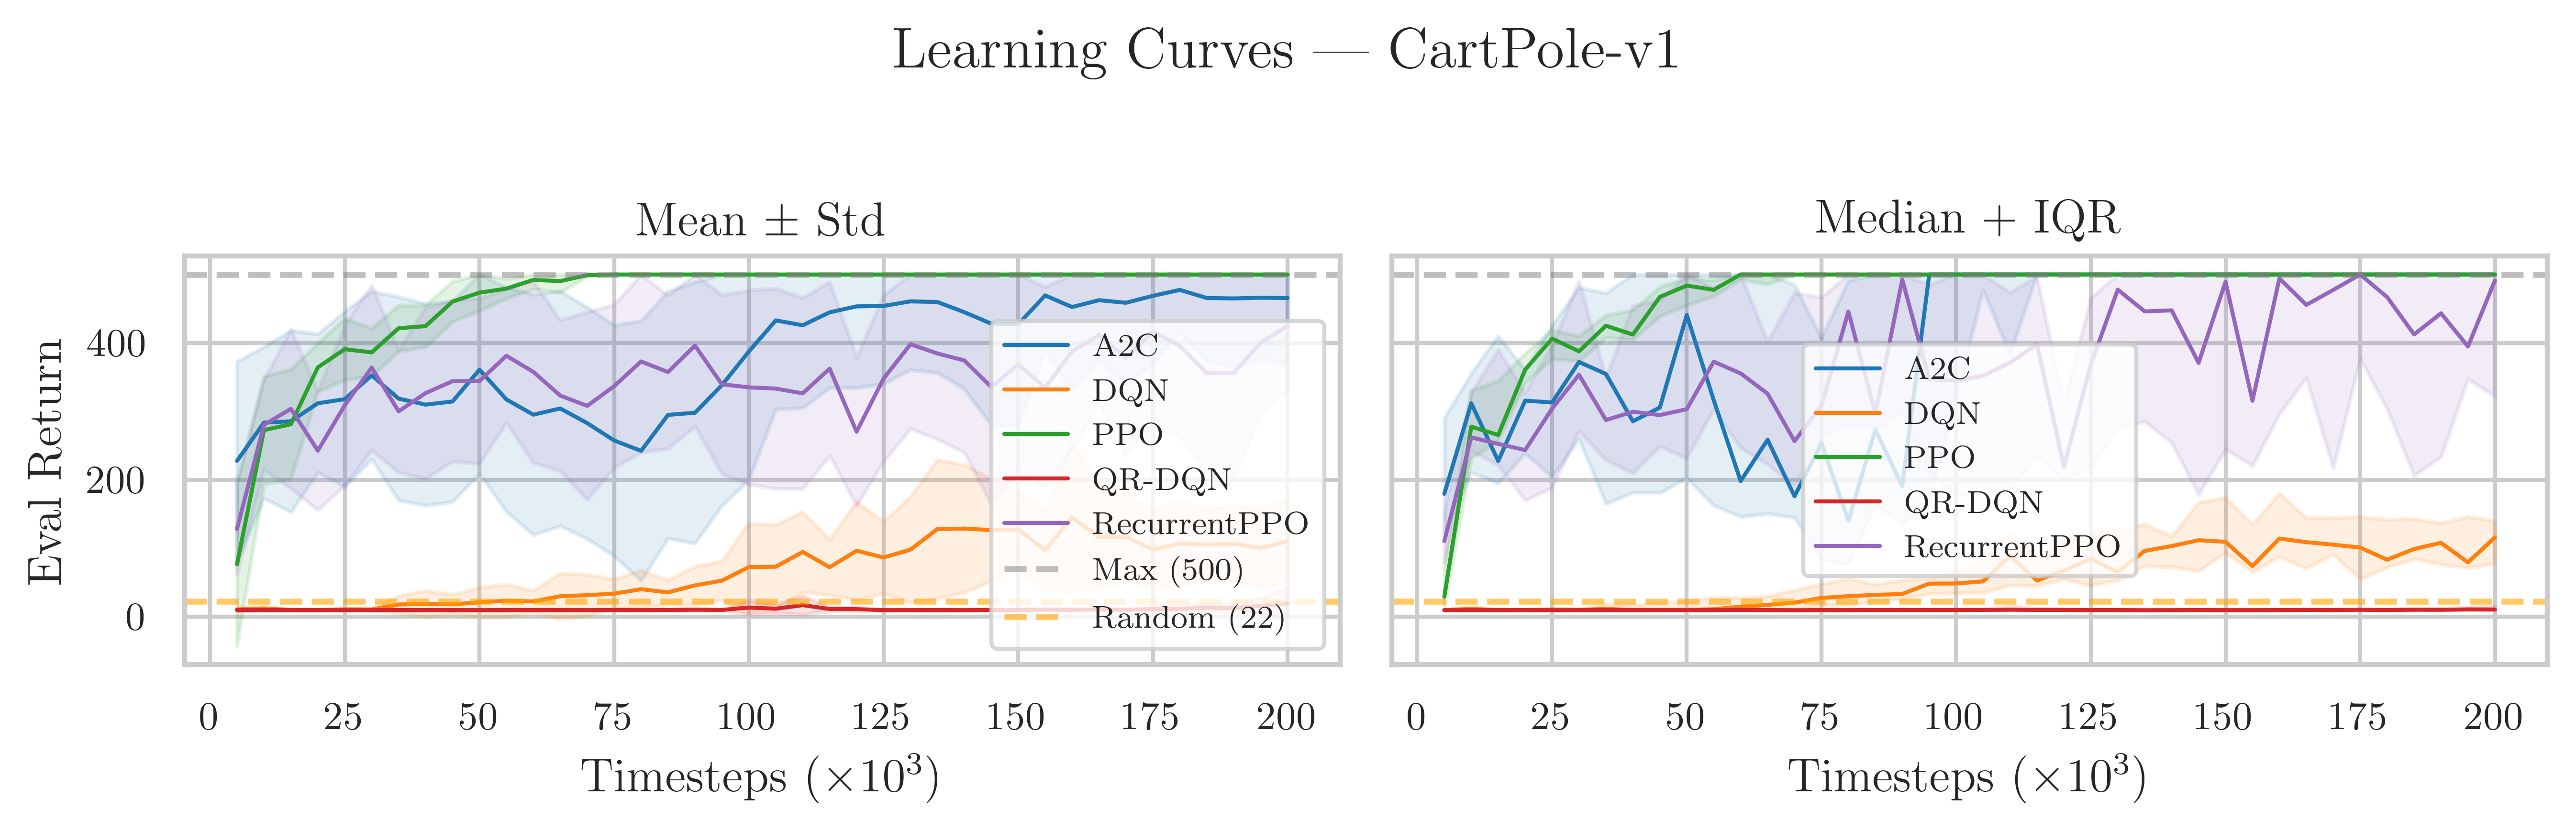
\includegraphics[width=\linewidth]{4_chapter/assets/learning_curves_cartpole-v1.png}
  \caption{Learning curves for CartPole-v1.  PPO and A2C converge to the
           maximum return of 500 within 100K steps.  DQN and QR-DQN fail to
           learn within the 200K-step budget.}
  \label{fig:lc-cartpole}
\end{figure}

\begin{figure}[ht]
  \centering
  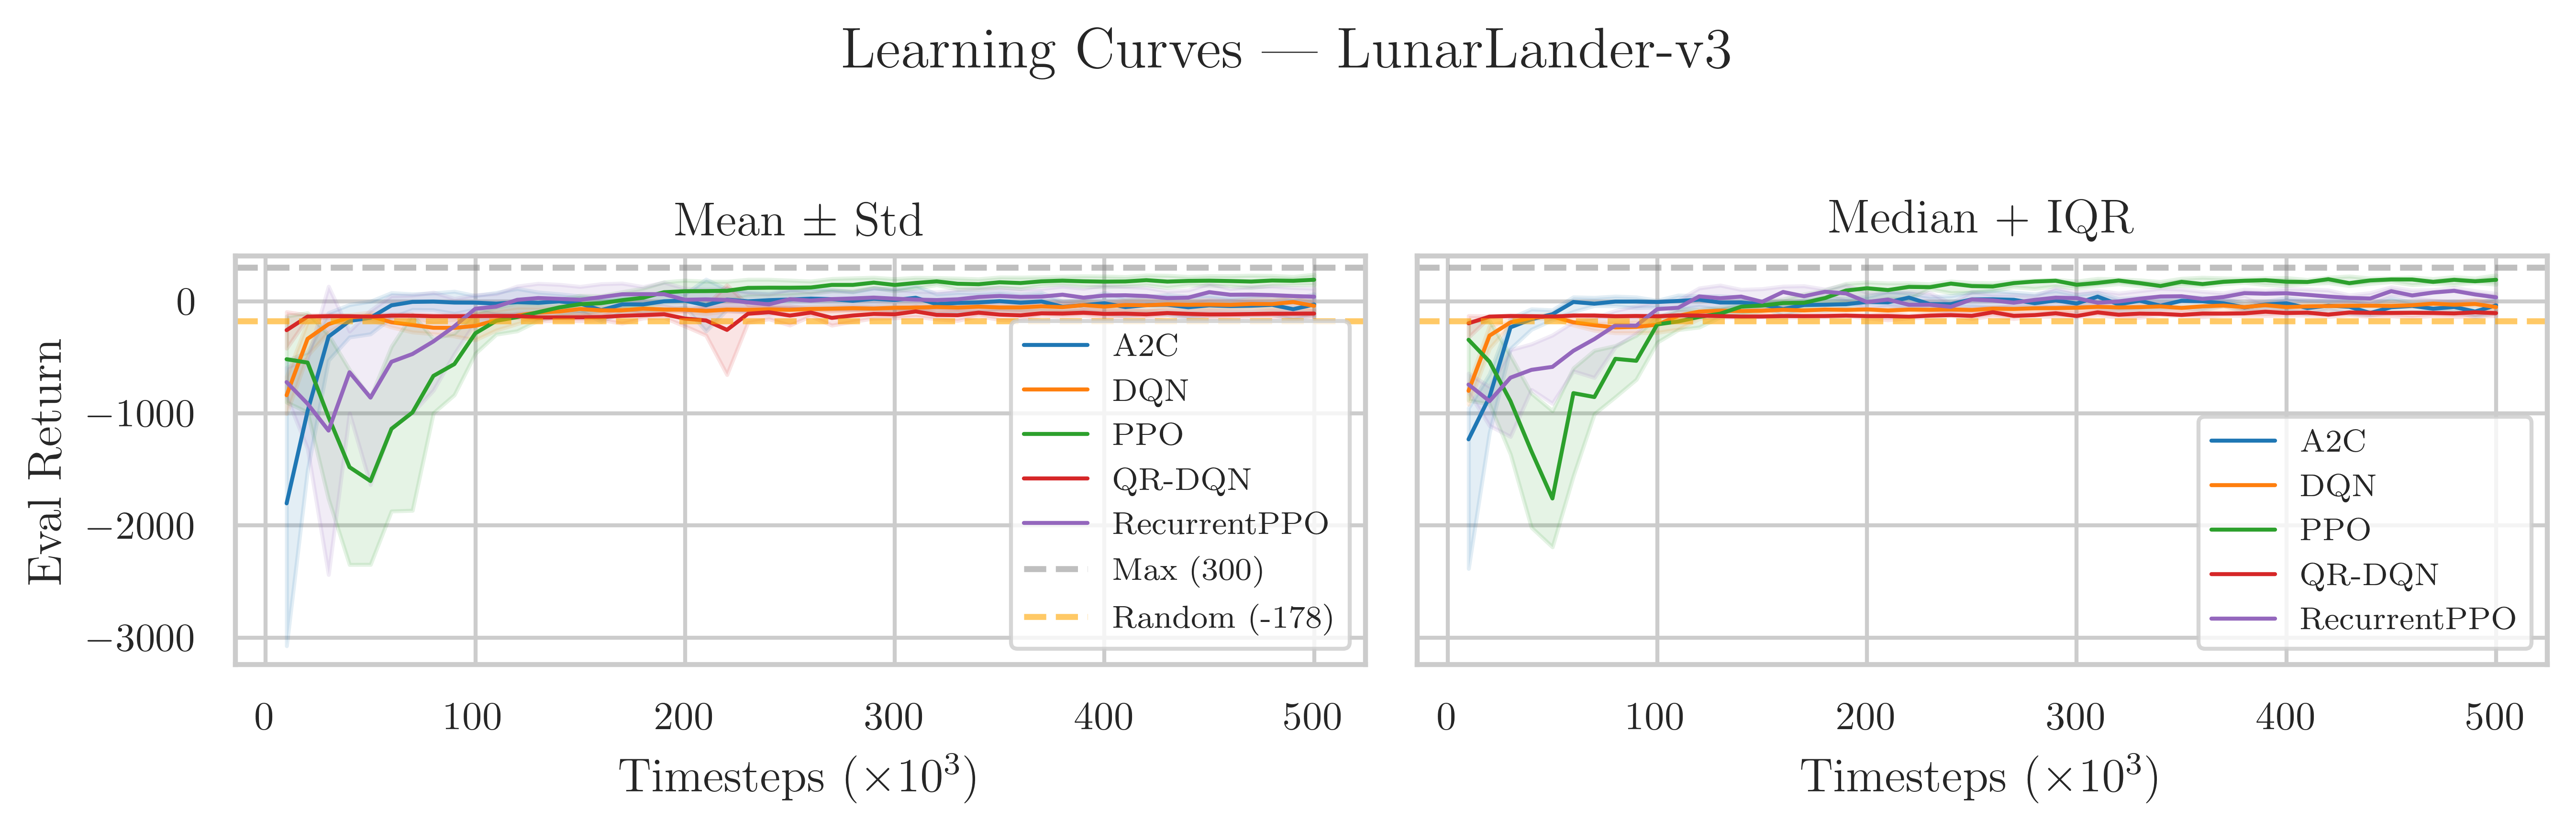
\includegraphics[width=\linewidth]{4_chapter/assets/learning_curves_lunarlander-v3.png}
  \caption{Learning curves for LunarLander-v3.  PPO achieves the highest
           median return ($\approx 230$).  A2C learns initially but exhibits
           high variance and eventual performance collapse.}
  \label{fig:lc-lunarlander}
\end{figure}

\begin{figure}[ht]
  \centering
  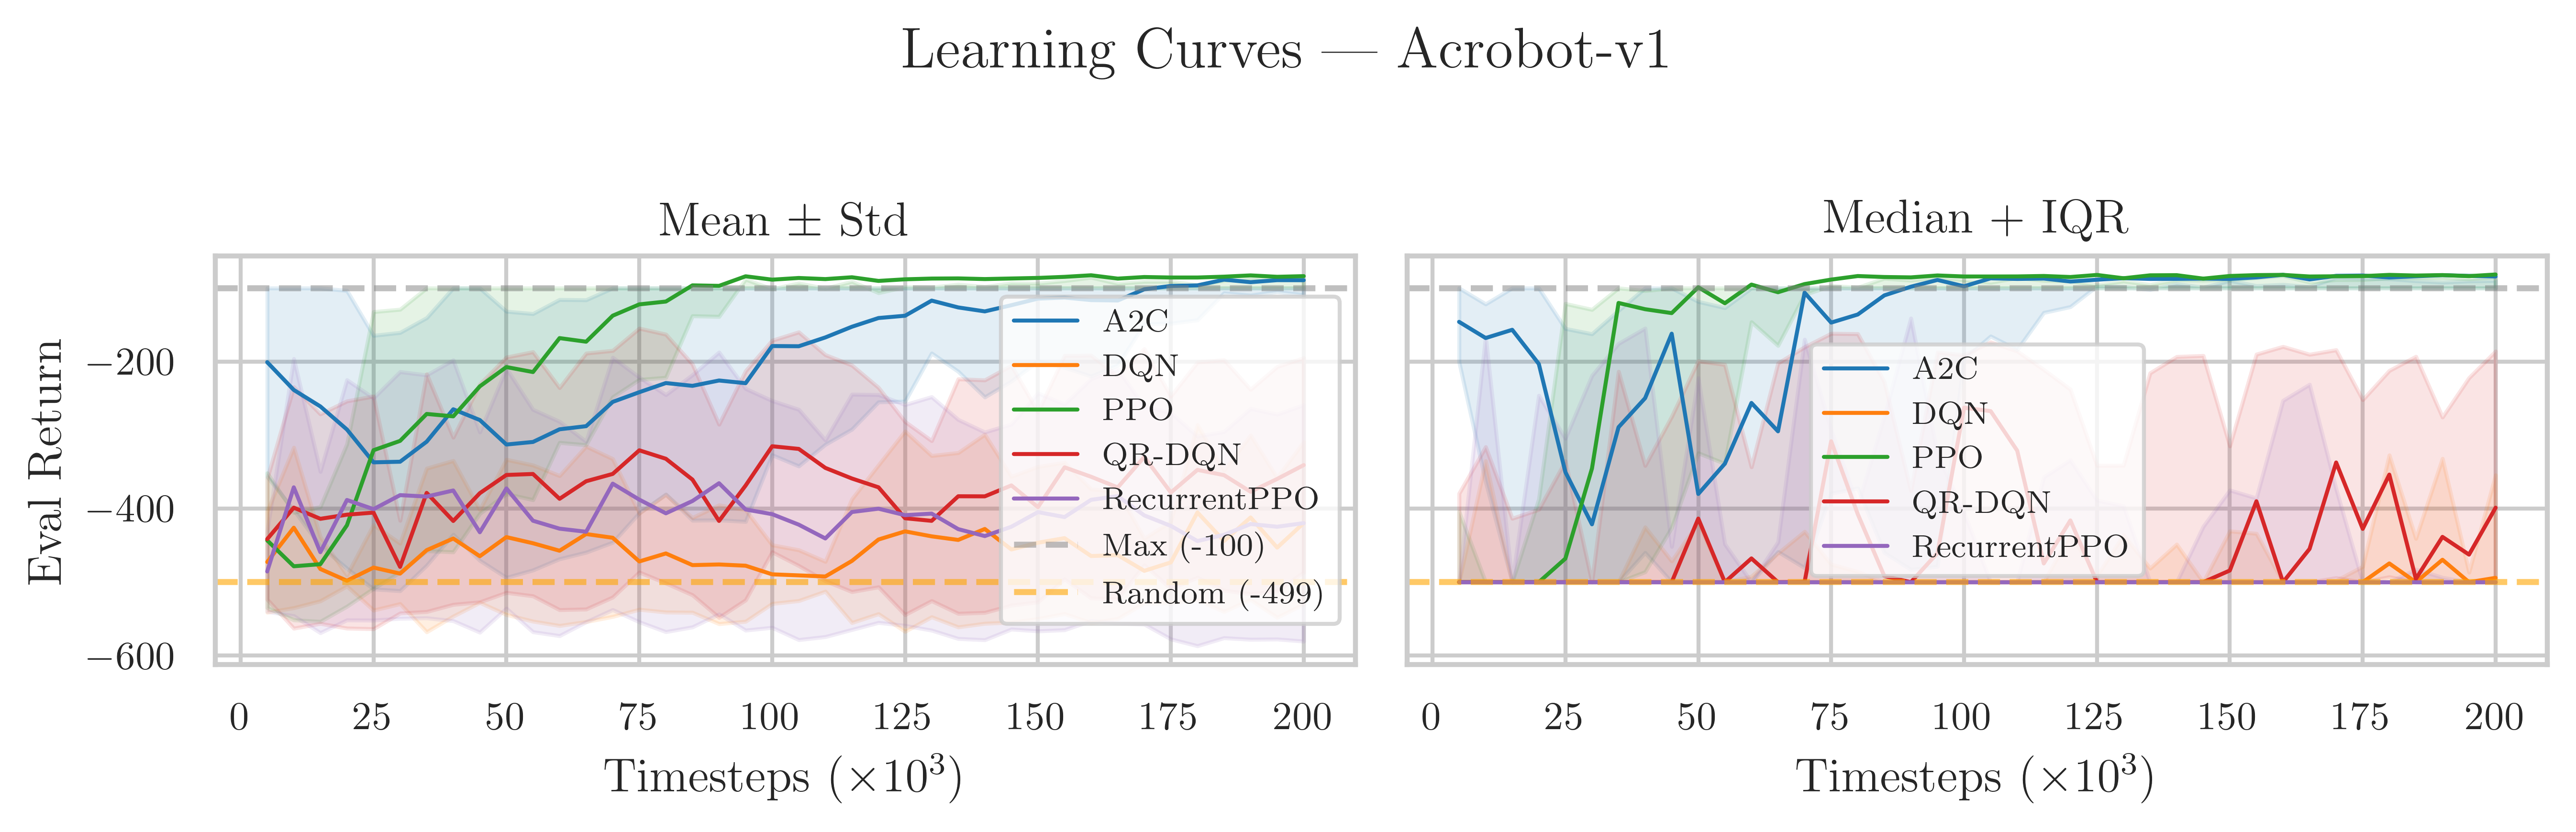
\includegraphics[width=\linewidth]{4_chapter/assets/learning_curves_acrobot-v1.png}
  \caption{Learning curves for Acrobot-v1.  A2C and PPO both converge
           near the optimal return ($\approx -85$).  RPPO fails entirely
           (median $\approx -500$, the episode truncation limit).}
  \label{fig:lc-acrobot}
\end{figure}

\begin{figure}[ht]
  \centering
  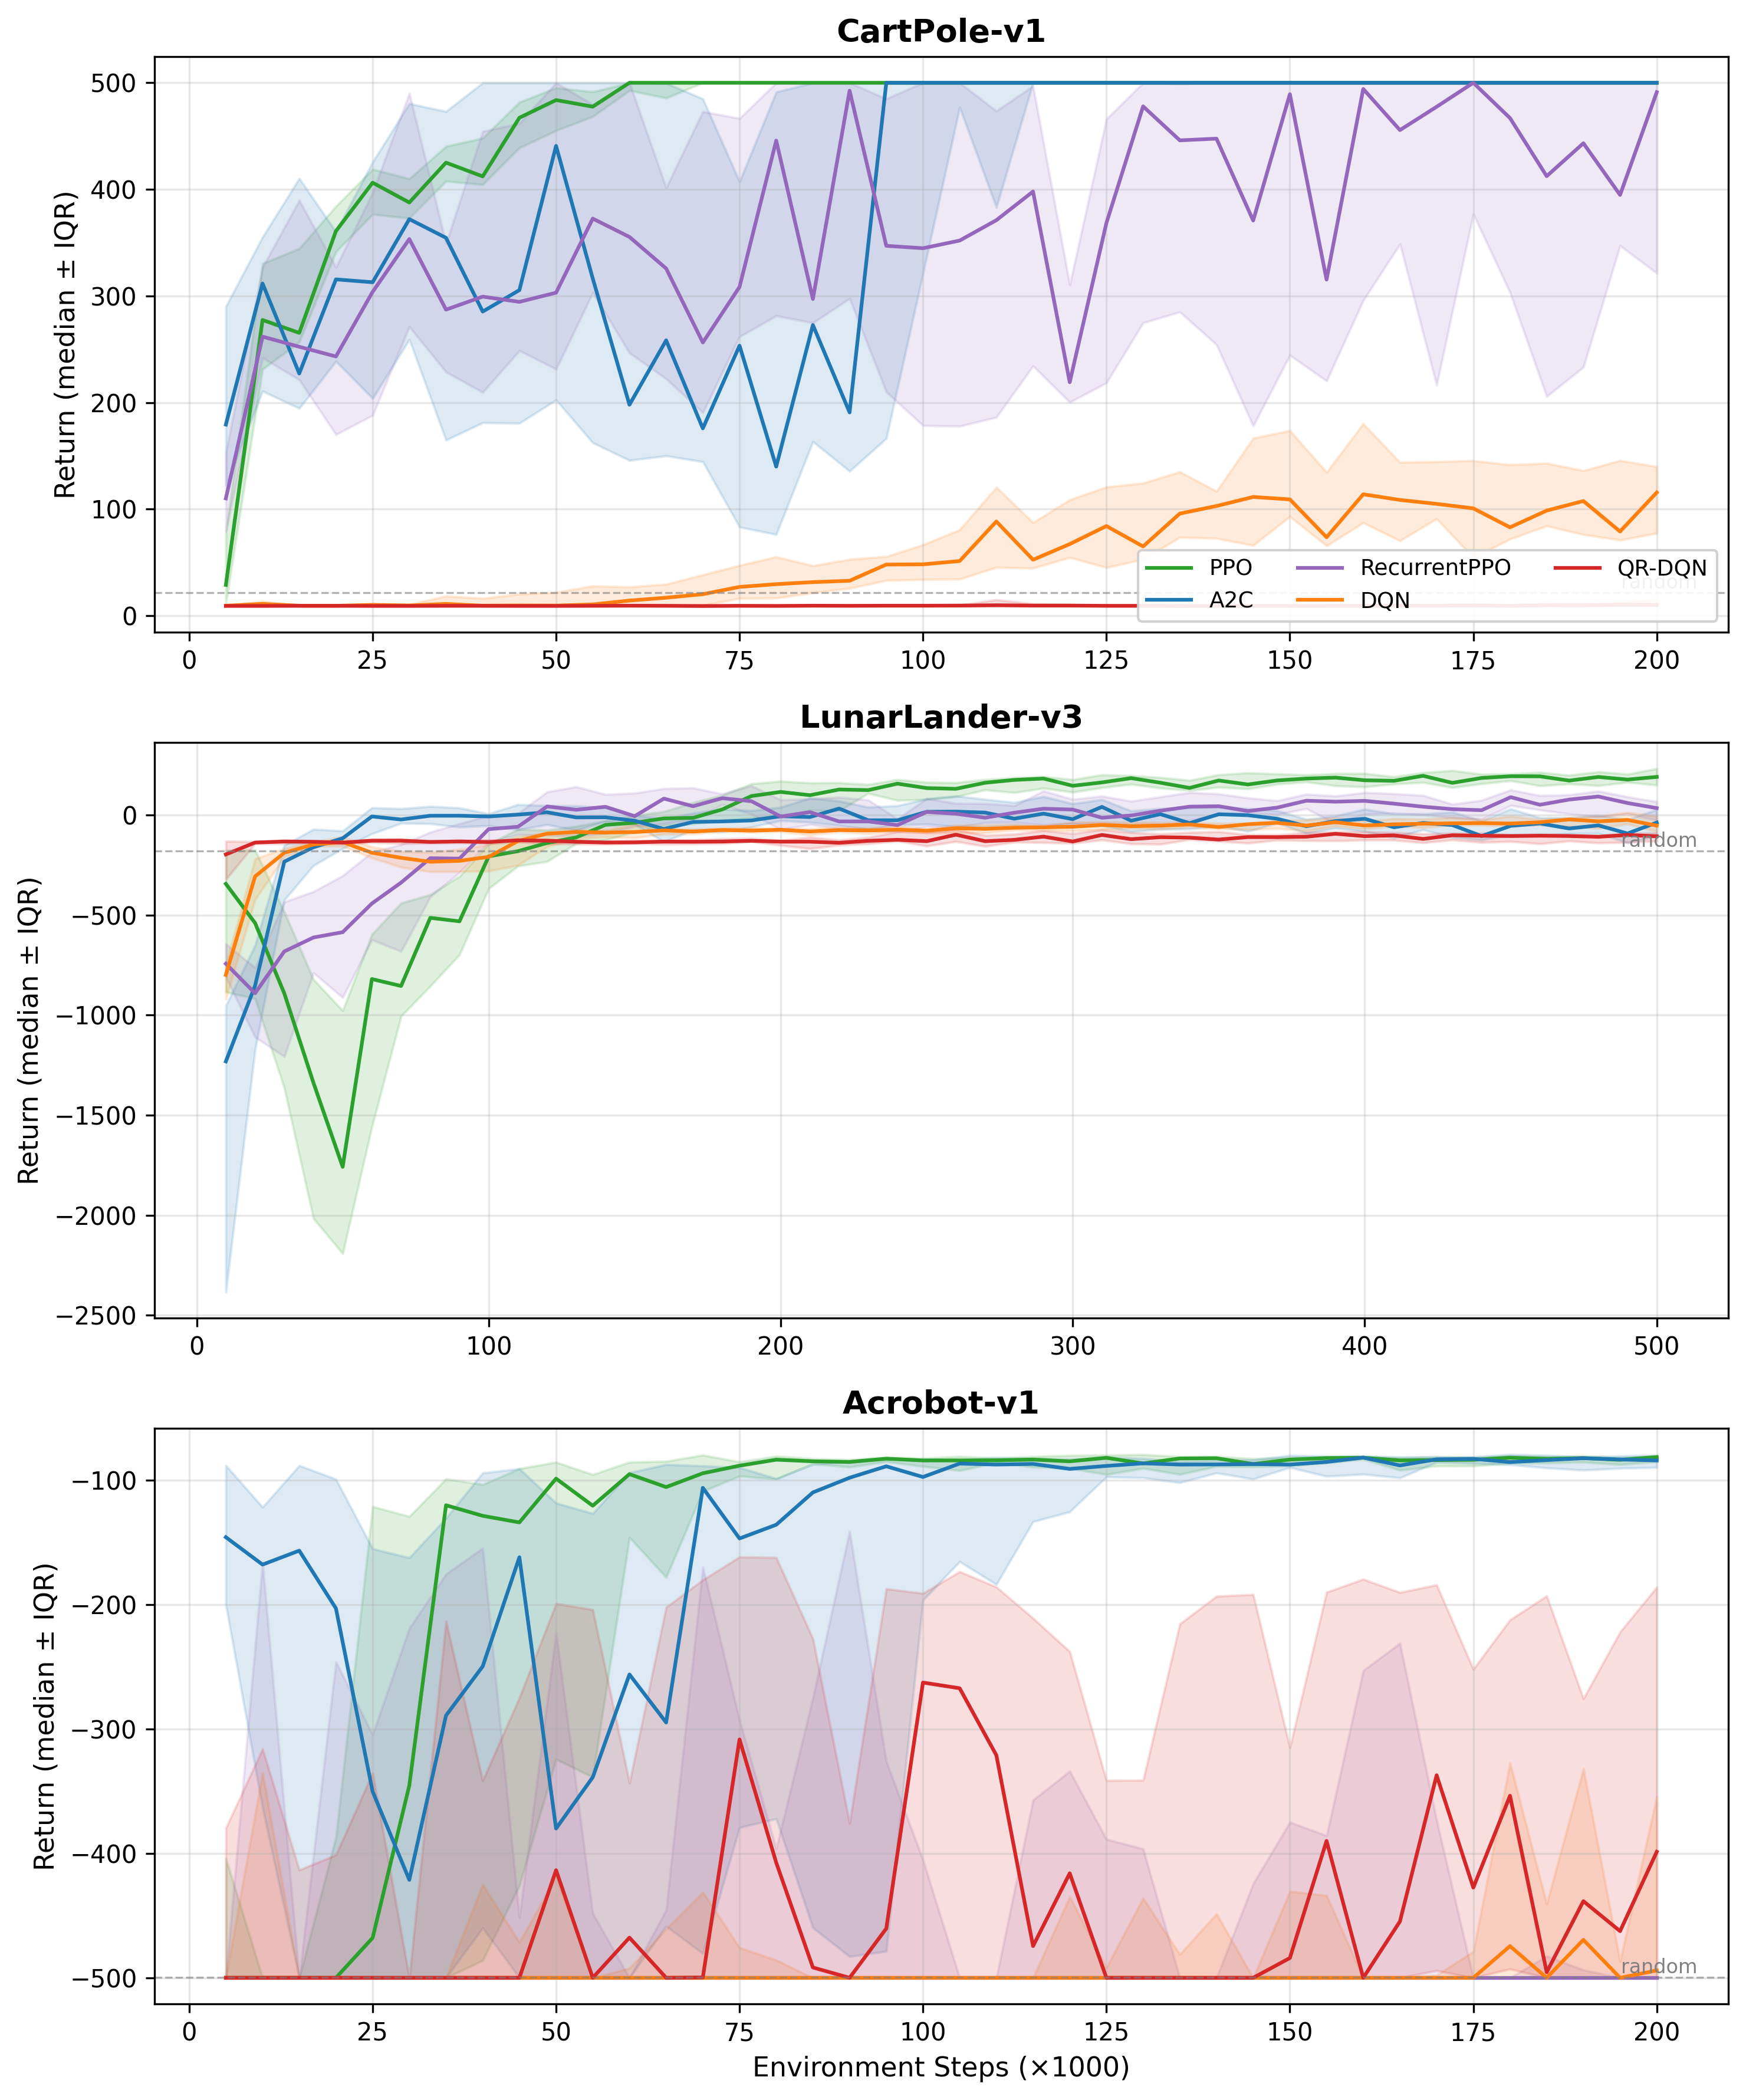
\includegraphics[width=\linewidth]{4_chapter/assets/combined_learning_curves.png}
  \caption{Combined normalised learning curves across all three
           environments.  PPO and A2C are the only algorithms that
           consistently rise above the random baseline across all tasks.}
  \label{fig:lc-combined}
\end{figure}

\paragraph{CartPole-v1.}
PPO achieves a perfect normalised IQM of $1.000$ $[1.000,\;1.000]$ with
zero variance: all 15 seeds reach the maximum return of 500.  A2C also
reaches IQM $1.000$ but with a wider confidence interval
$[0.926,\;1.000]$, indicating that some seeds converge slower.
The DQN-family algorithms (DQN: $0.175$; QR-DQN: $-0.022$) fail almost
entirely under the 200K-step budget, with QR-DQN scoring below the random
baseline.

\paragraph{LunarLander-v3.}
This is the hardest environment in our suite.  PPO leads with IQM
$0.768$ $[0.714,\;0.814]$.  Notably, RPPO ($0.444$) outperforms
A2C ($0.303$) and DQN ($0.309$), likely because the LSTM can exploit
temporal correlations in the lander's trajectory.  QR-DQN achieves
IQM $0.146$, the lowest score on this environment.

\paragraph{Acrobot-v1.}
PPO and A2C both achieve normalised IQM above 1.0 (PPO: $1.039$,
A2C: $1.040$), meaning they consistently beat the reference maximum return.
RPPO catastrophically fails (IQM $-0.001$), with most seeds stuck at the
truncation limit of $-500$.  This is likely because the LSTM adds
unnecessary complexity to a fully-observed Markov environment, impairing
optimisation.

\subsection{Score Distributions and Per-Seed Analysis}
\label{sec:score-dist}

Figure~\ref{fig:score-dist} shows the distribution of normalised final
scores across all $N \times M = 45$ seed--environment pairs per algorithm.
Figures~\ref{fig:heatmap} and~\ref{fig:boxswarm} provide complementary
per-seed views: a heatmap of normalised scores and a box-and-swarm plot
with anomaly detection.

\begin{figure}[ht]
  \centering
  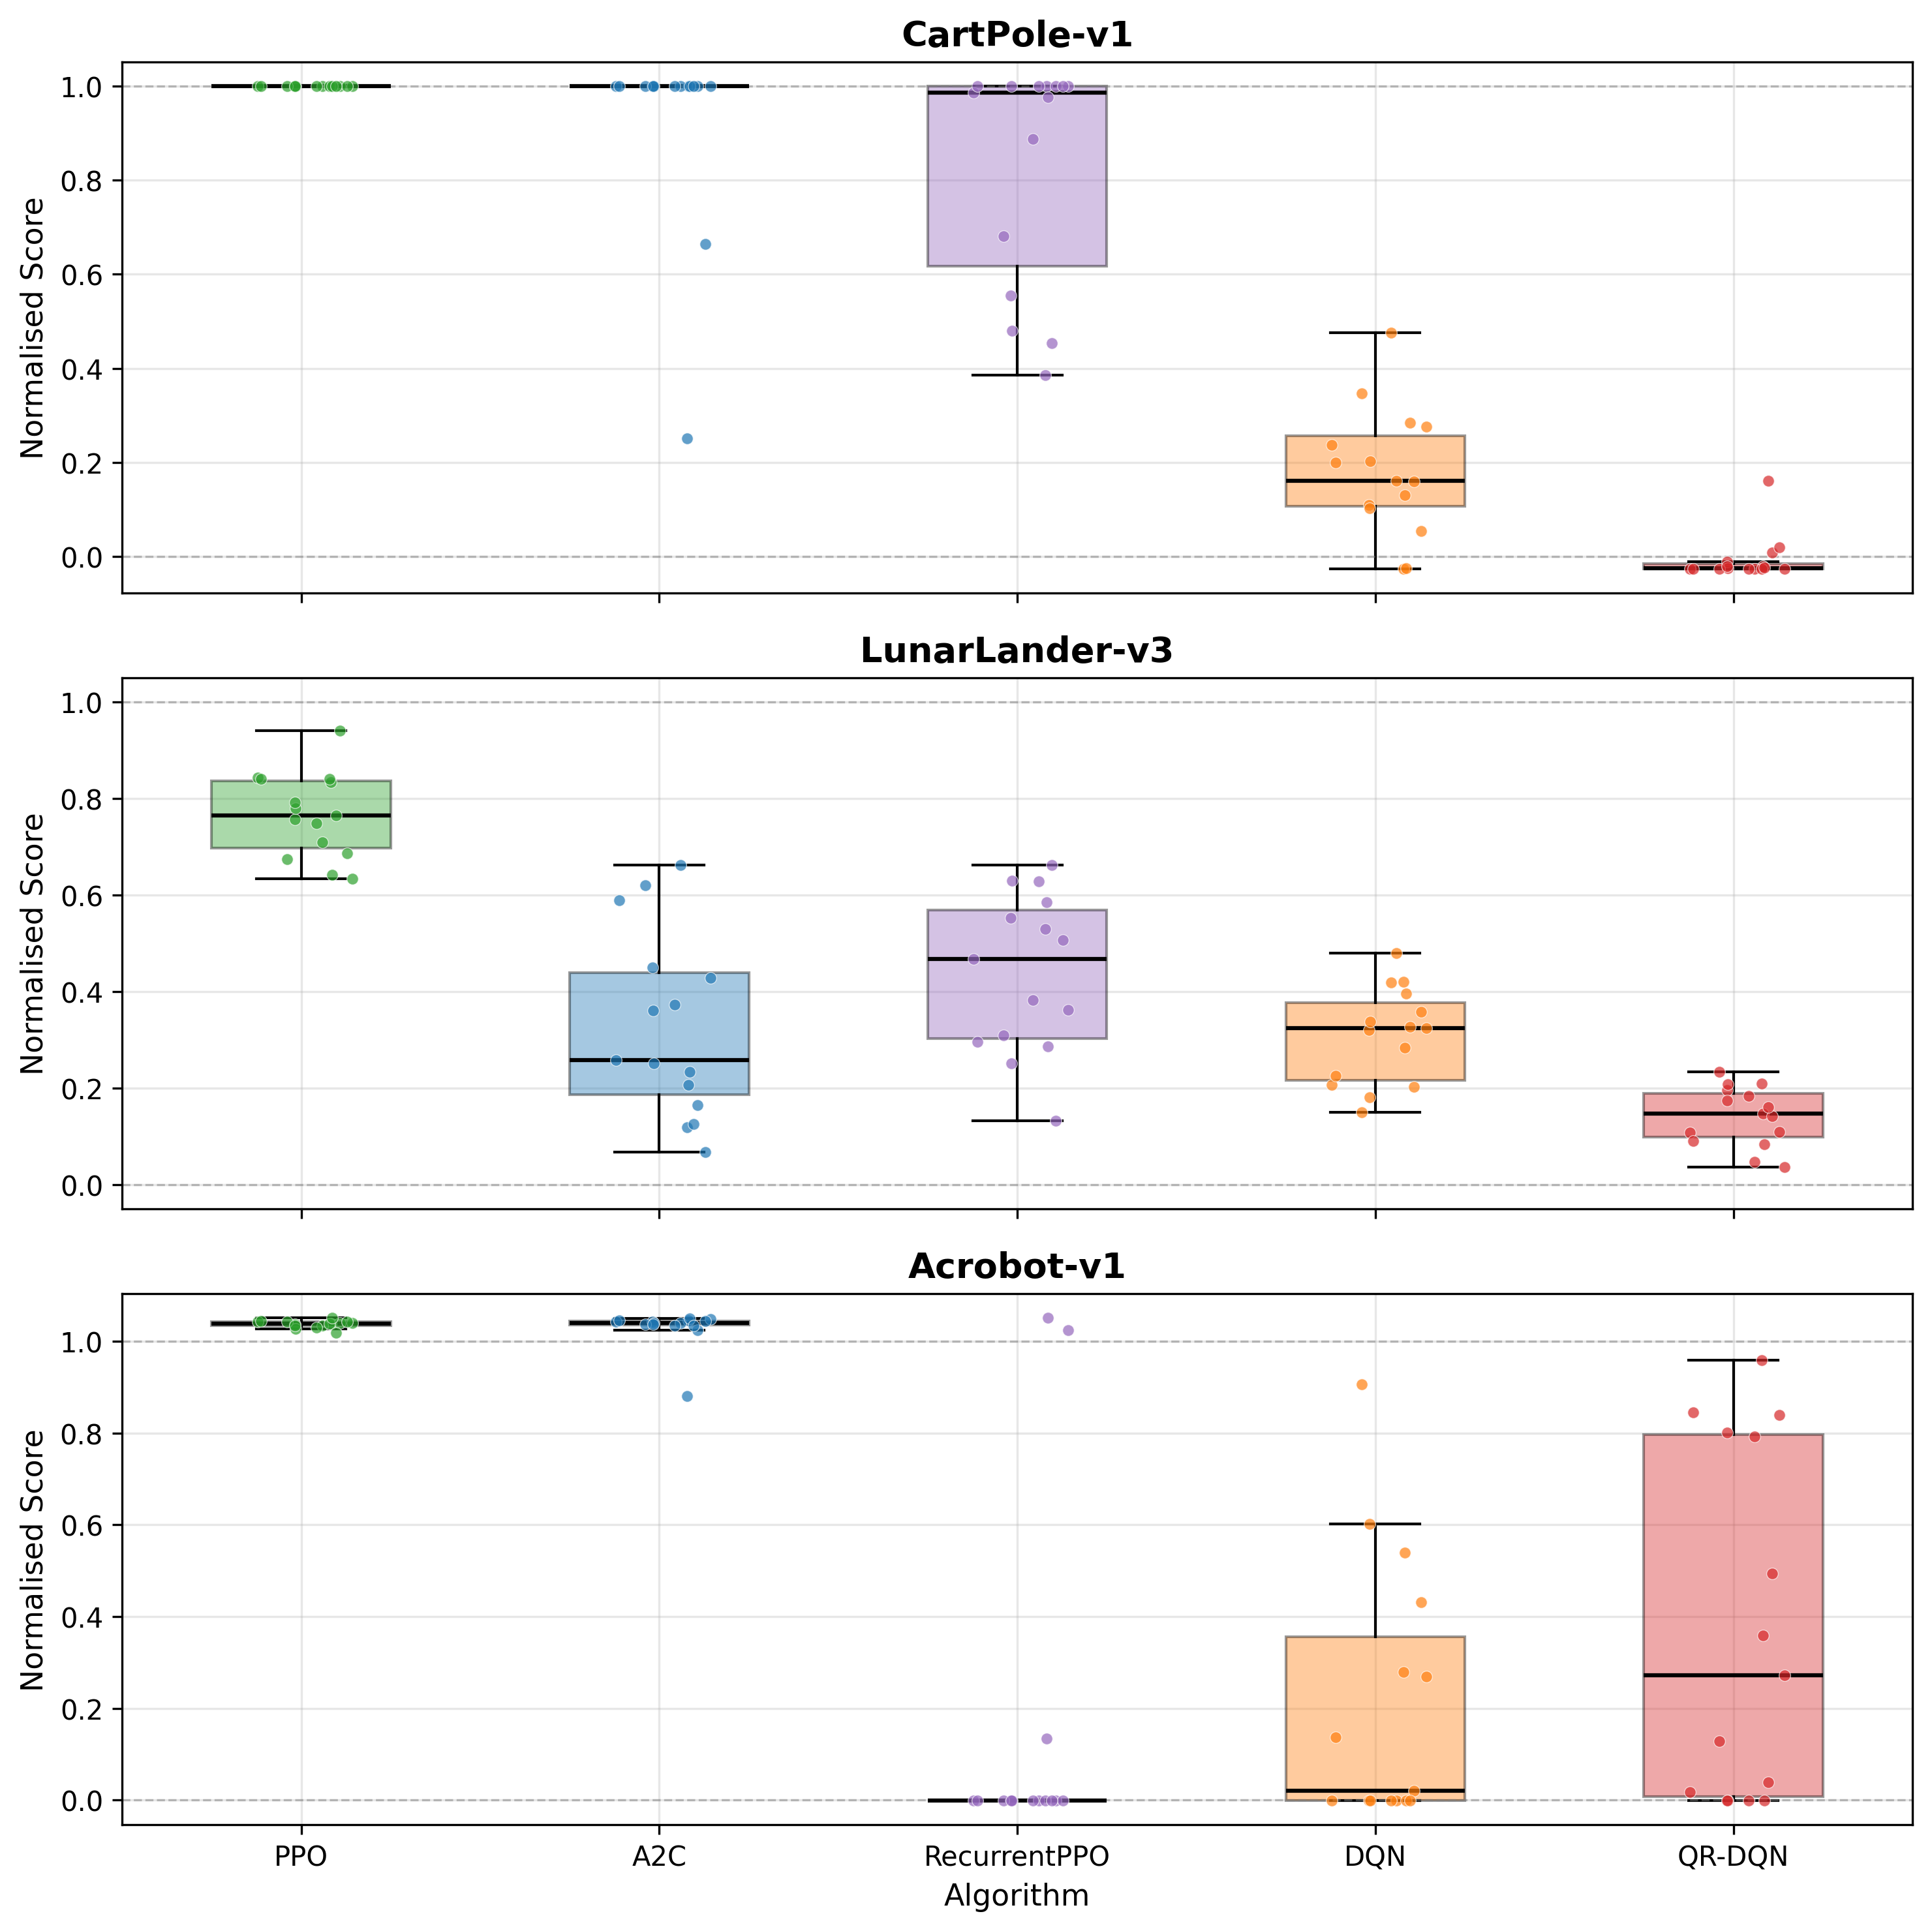
\includegraphics[width=\linewidth]{4_chapter/assets/score_distribution.png}
  \caption{Distribution of normalised scores across all seed--environment
           pairs.  PPO is concentrated near 1.0; A2C is bimodal (strong on
           CartPole and Acrobot, weak on LunarLander); DQN and QR-DQN are
           concentrated near zero.}
  \label{fig:score-dist}
\end{figure}

\begin{figure}[ht]
  \centering
  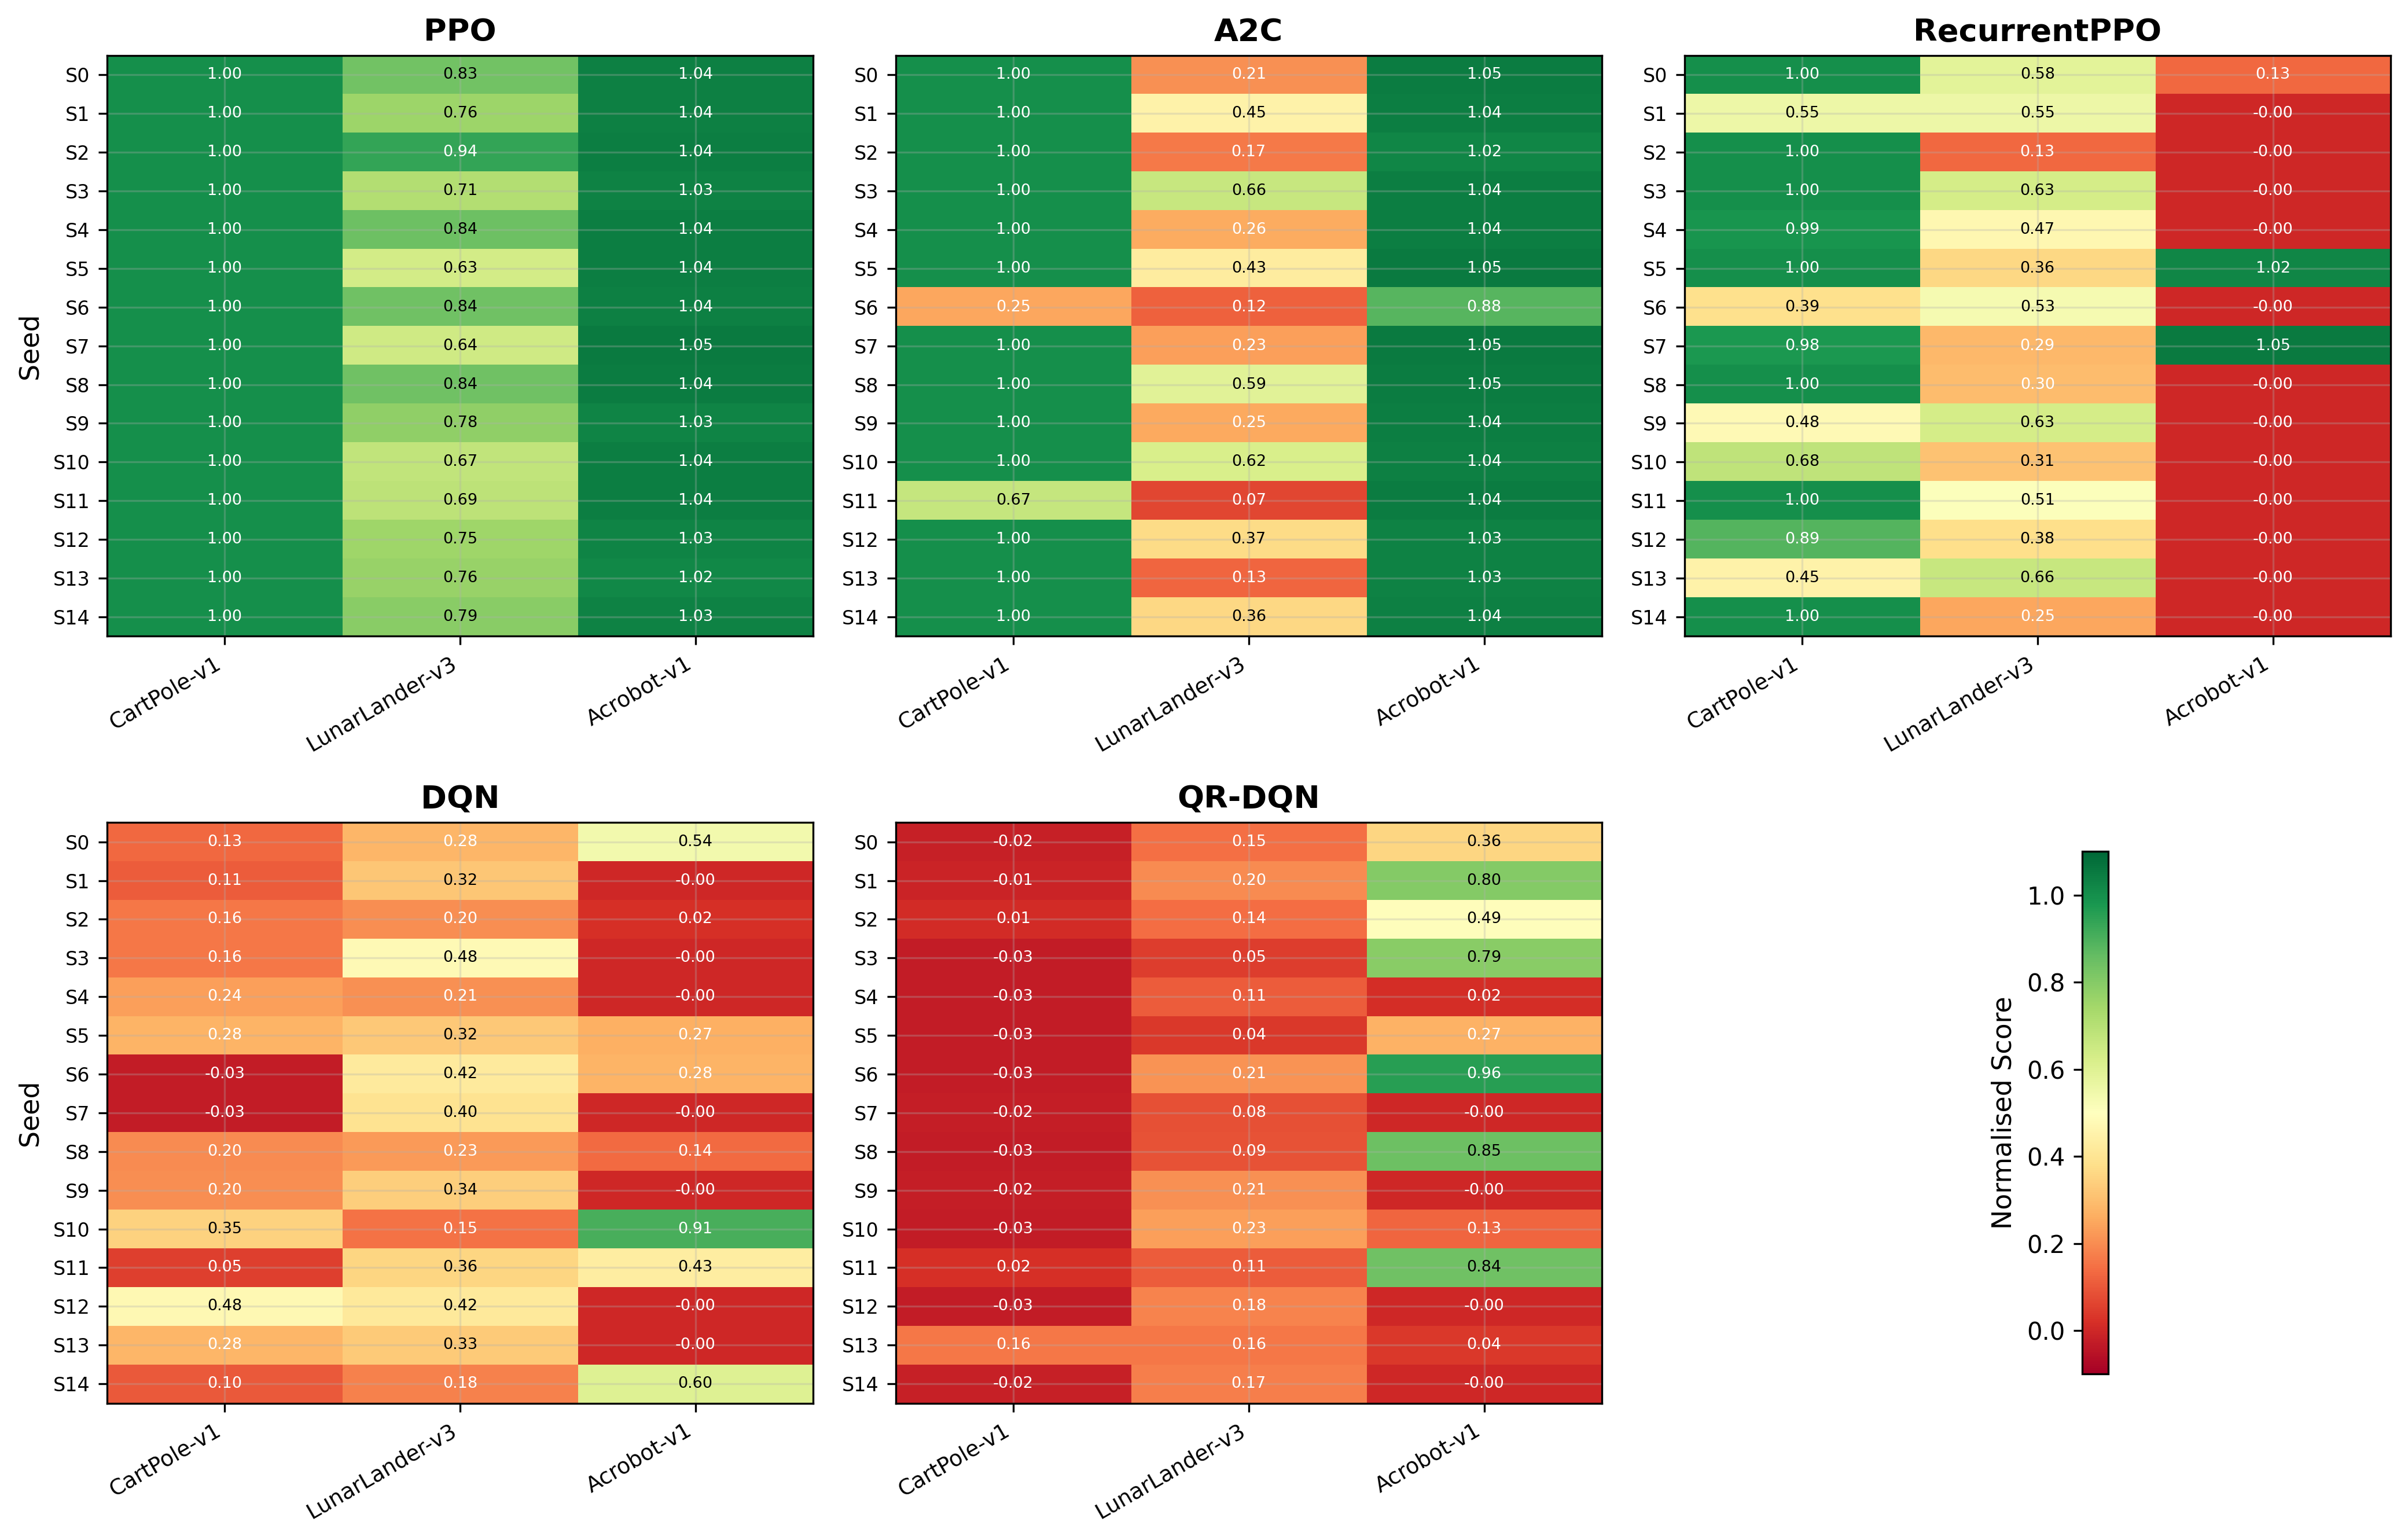
\includegraphics[width=\linewidth]{4_chapter/assets/per_seed_heatmap.png}
  \caption{Heatmap of normalised final scores by seed and environment.
           Each row is one of the 15 seeds; columns are environments.
           PPO achieves uniformly high scores.  RPPO shows a clear
           environment-dependent failure mode on Acrobot.}
  \label{fig:heatmap}
\end{figure}

\begin{figure}[ht]
  \centering
  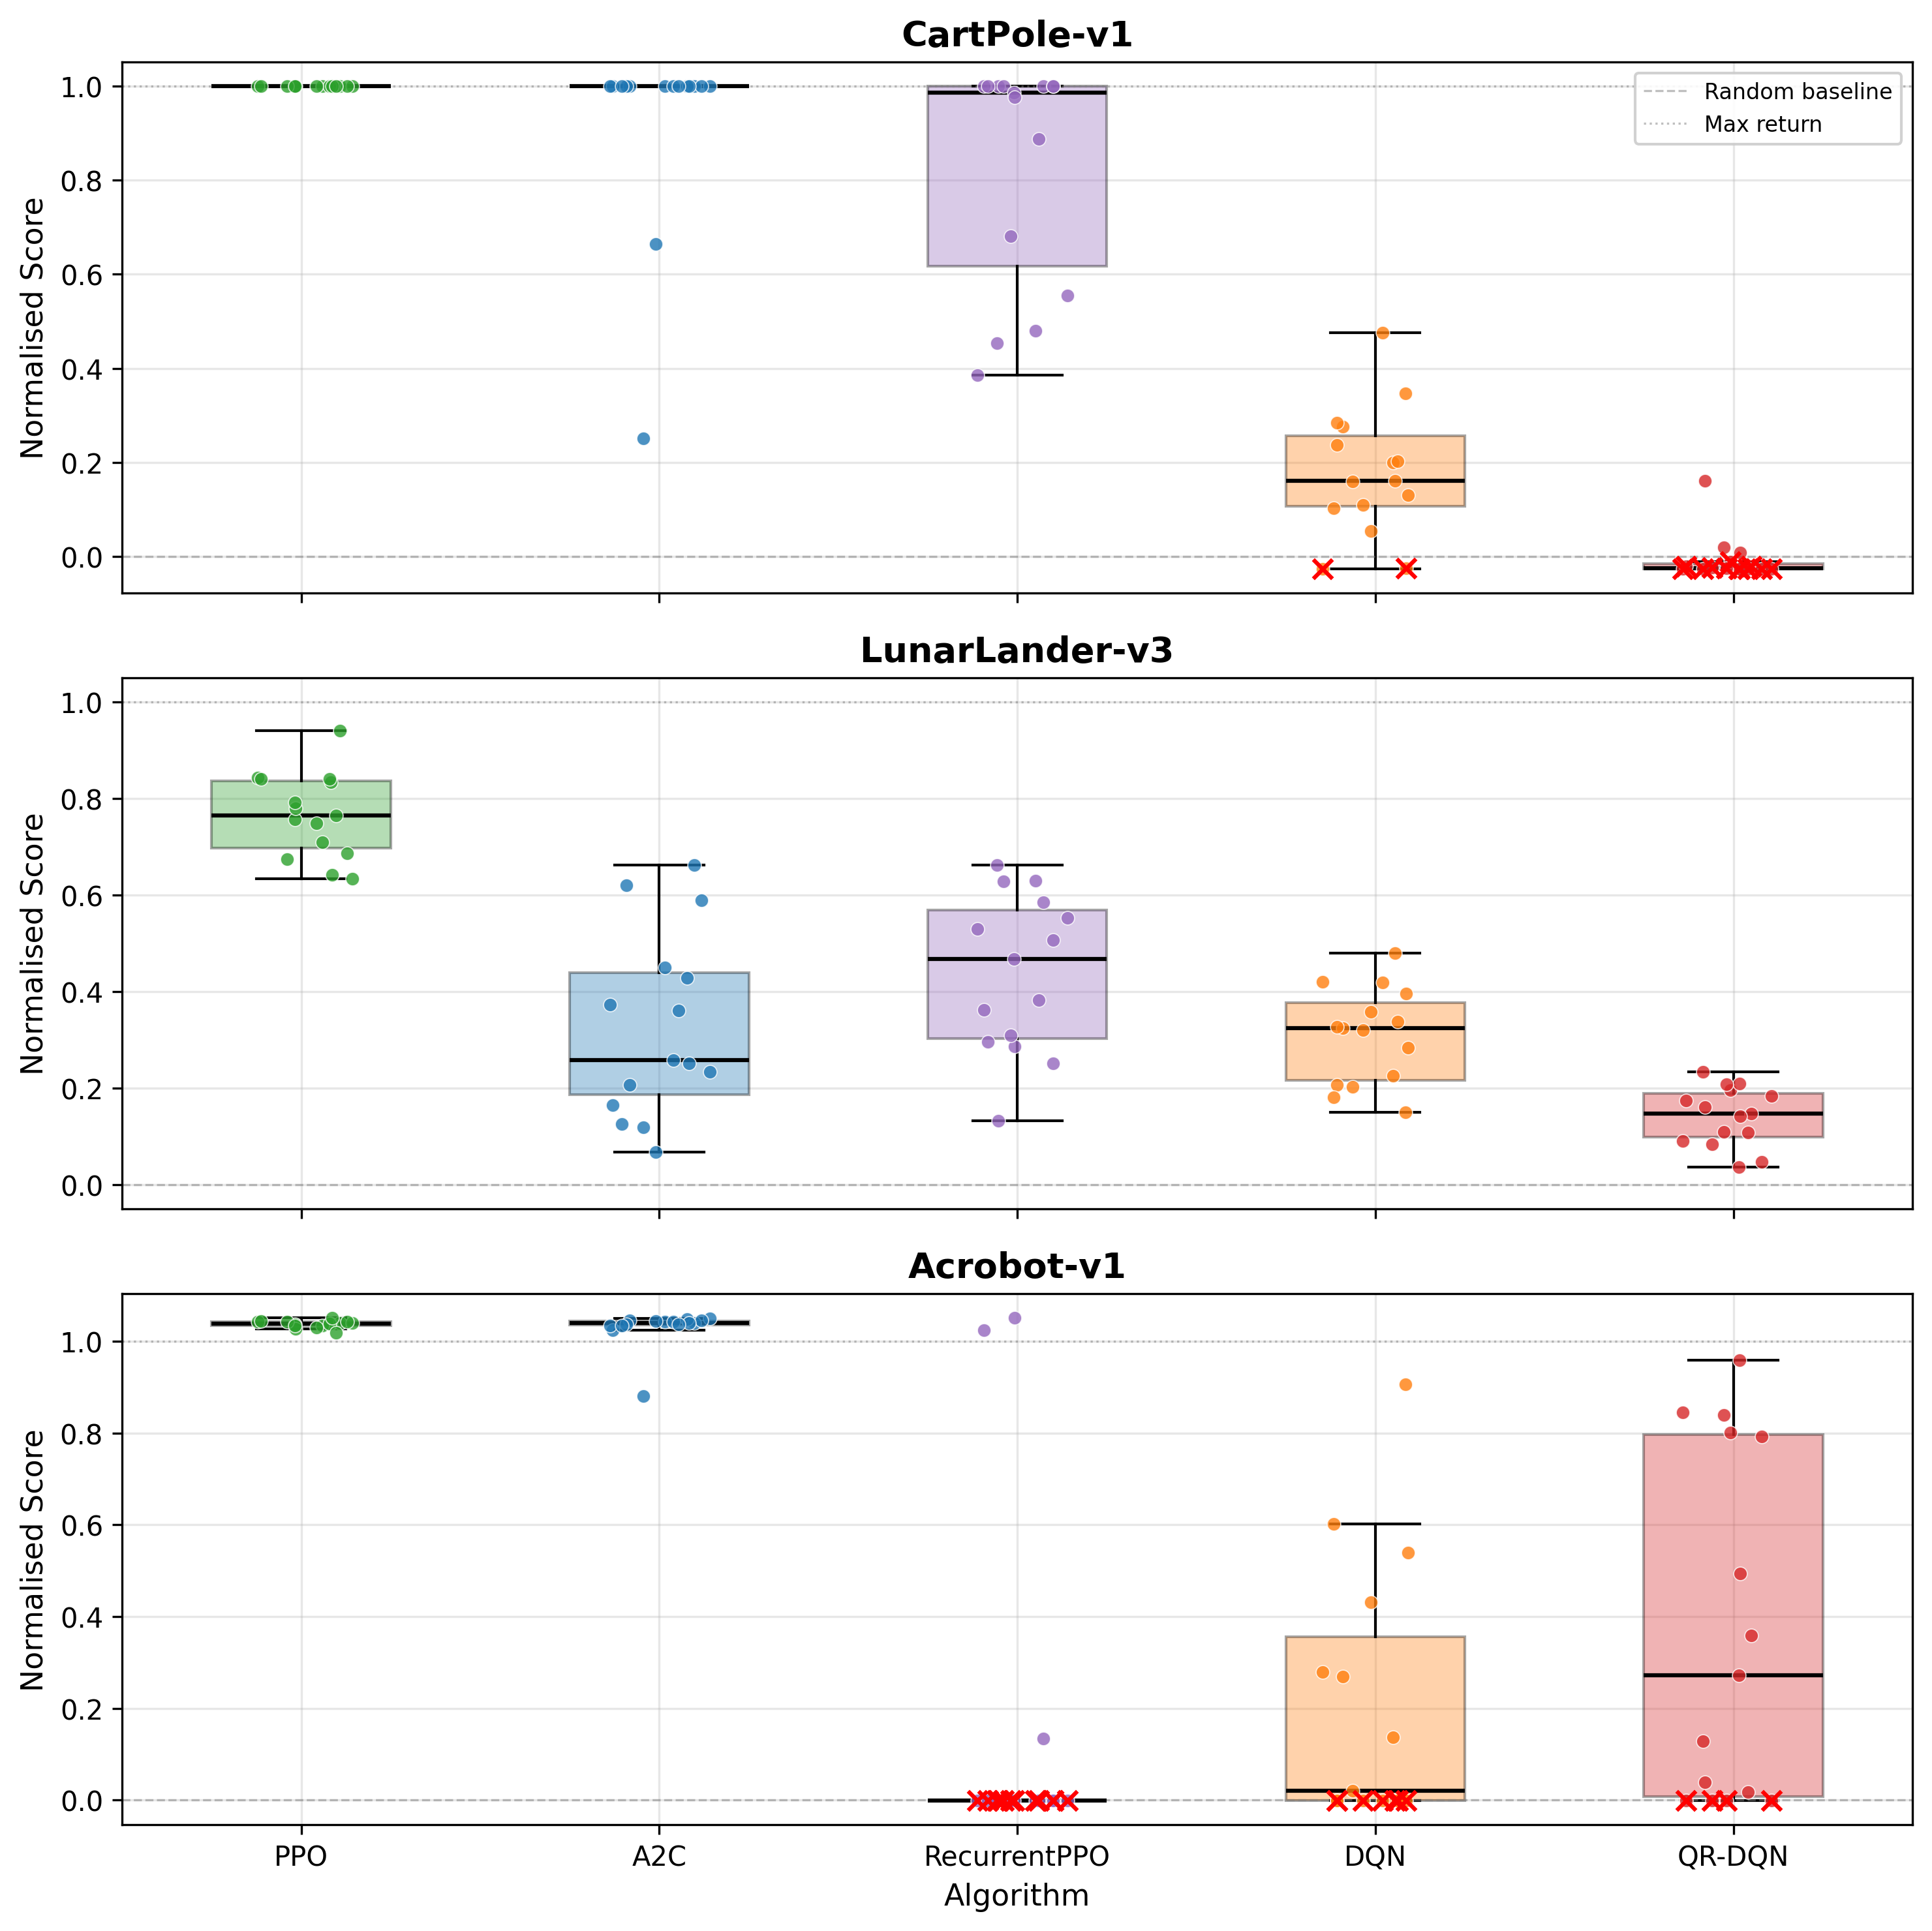
\includegraphics[width=\linewidth]{4_chapter/assets/per_seed_boxswarm.png}
  \caption{Box-and-swarm plot of per-seed normalised scores.  Individual
           seeds are shown as dots; boxes indicate the IQR.  A2C exhibits
           the widest spread on LunarLander; PPO has near-zero variance
           on CartPole and Acrobot.}
  \label{fig:boxswarm}
\end{figure}

Table~\ref{tab:per-env-iqm} summarises the per-environment normalised
IQM with 95\% bootstrap confidence intervals.

\begin{table}[ht]
\centering
\caption{Per-environment normalised IQM with 95\% bootstrap CIs.}
\label{tab:per-env-iqm}
\begin{tabular}{lccc}
\toprule
\textbf{Algorithm} & \textbf{CartPole-v1} & \textbf{LunarLander-v3}
                   & \textbf{Acrobot-v1} \\
\midrule
PPO    & $1.000\;[1.000,\;1.000]$ & $0.768\;[0.714,\;0.814]$
       & $1.039\;[1.034,\;1.042]$ \\
A2C    & $1.000\;[0.926,\;1.000]$ & $0.303\;[0.204,\;0.438]$
       & $1.040\;[1.035,\;1.044]$ \\
RPPO   & $0.898\;[0.704,\;0.997]$ & $0.444\;[0.343,\;0.548]$
       & $-0.001\;[-0.001,\;0.241]$ \\
DQN    & $0.175\;[0.104,\;0.242]$ & $0.309\;[0.249,\;0.368]$
       & $0.126\;[0.003,\;0.328]$ \\
QR-DQN & $-0.022\;[-0.025,\;-0.007]$ & $0.146\;[0.107,\;0.181]$
       & $0.322\;[0.077,\;0.622]$ \\
\bottomrule
\end{tabular}
\end{table}

%% ------------------------------------------------------------------
\section{Cross-Environment Aggregate Results}
\label{sec:cross-env-results}

\subsection{Final Performance}
\label{sec:final-perf}

Table~\ref{tab:cross-env} reports the cross-environment aggregate metrics
at the final training budget.  PPO achieves the highest IQM ($0.981$) with
the tightest confidence interval and the smallest optimality gap ($0.078$).

\begin{table}[ht]
\centering
\caption{Cross-environment aggregate metrics (normalised scores).  IQM,
         mean, and median are reported with 95\% bootstrap CIs.}
\label{tab:cross-env}
\begin{tabular}{lcccc}
\toprule
\textbf{Algorithm} & \textbf{IQM} & \textbf{Mean} & \textbf{Median}
                   & \textbf{Opt.\ Gap} \\
\midrule
PPO    & $0.981\;[0.971,\;0.991]$ & $0.934\;[0.912,\;0.953]$
       & $1.000$ & $0.078\;[0.064,\;0.092]$ \\
A2C    & $0.886\;[0.807,\;0.934]$ & $0.762\;[0.713,\;0.805]$
       & $0.928$ & $0.251\;[0.208,\;0.299]$ \\
RPPO   & $0.442\;[0.345,\;0.583]$ & $0.471\;[0.382,\;0.556]$
       & $0.439$ & $0.531\;[0.454,\;0.601]$ \\
DQN    & $0.222\;[0.164,\;0.276]$ & $0.233\;[0.186,\;0.280]$
       & $0.212$ & $0.767\;[0.710,\;0.818]$ \\
QR-DQN & $0.080\;[0.045,\;0.121]$ & $0.168\;[0.115,\;0.225]$
       & $0.142$ & $0.832\;[0.768,\;0.893]$ \\
\bottomrule
\end{tabular}
\end{table}

\begin{figure}[ht]
  \centering
  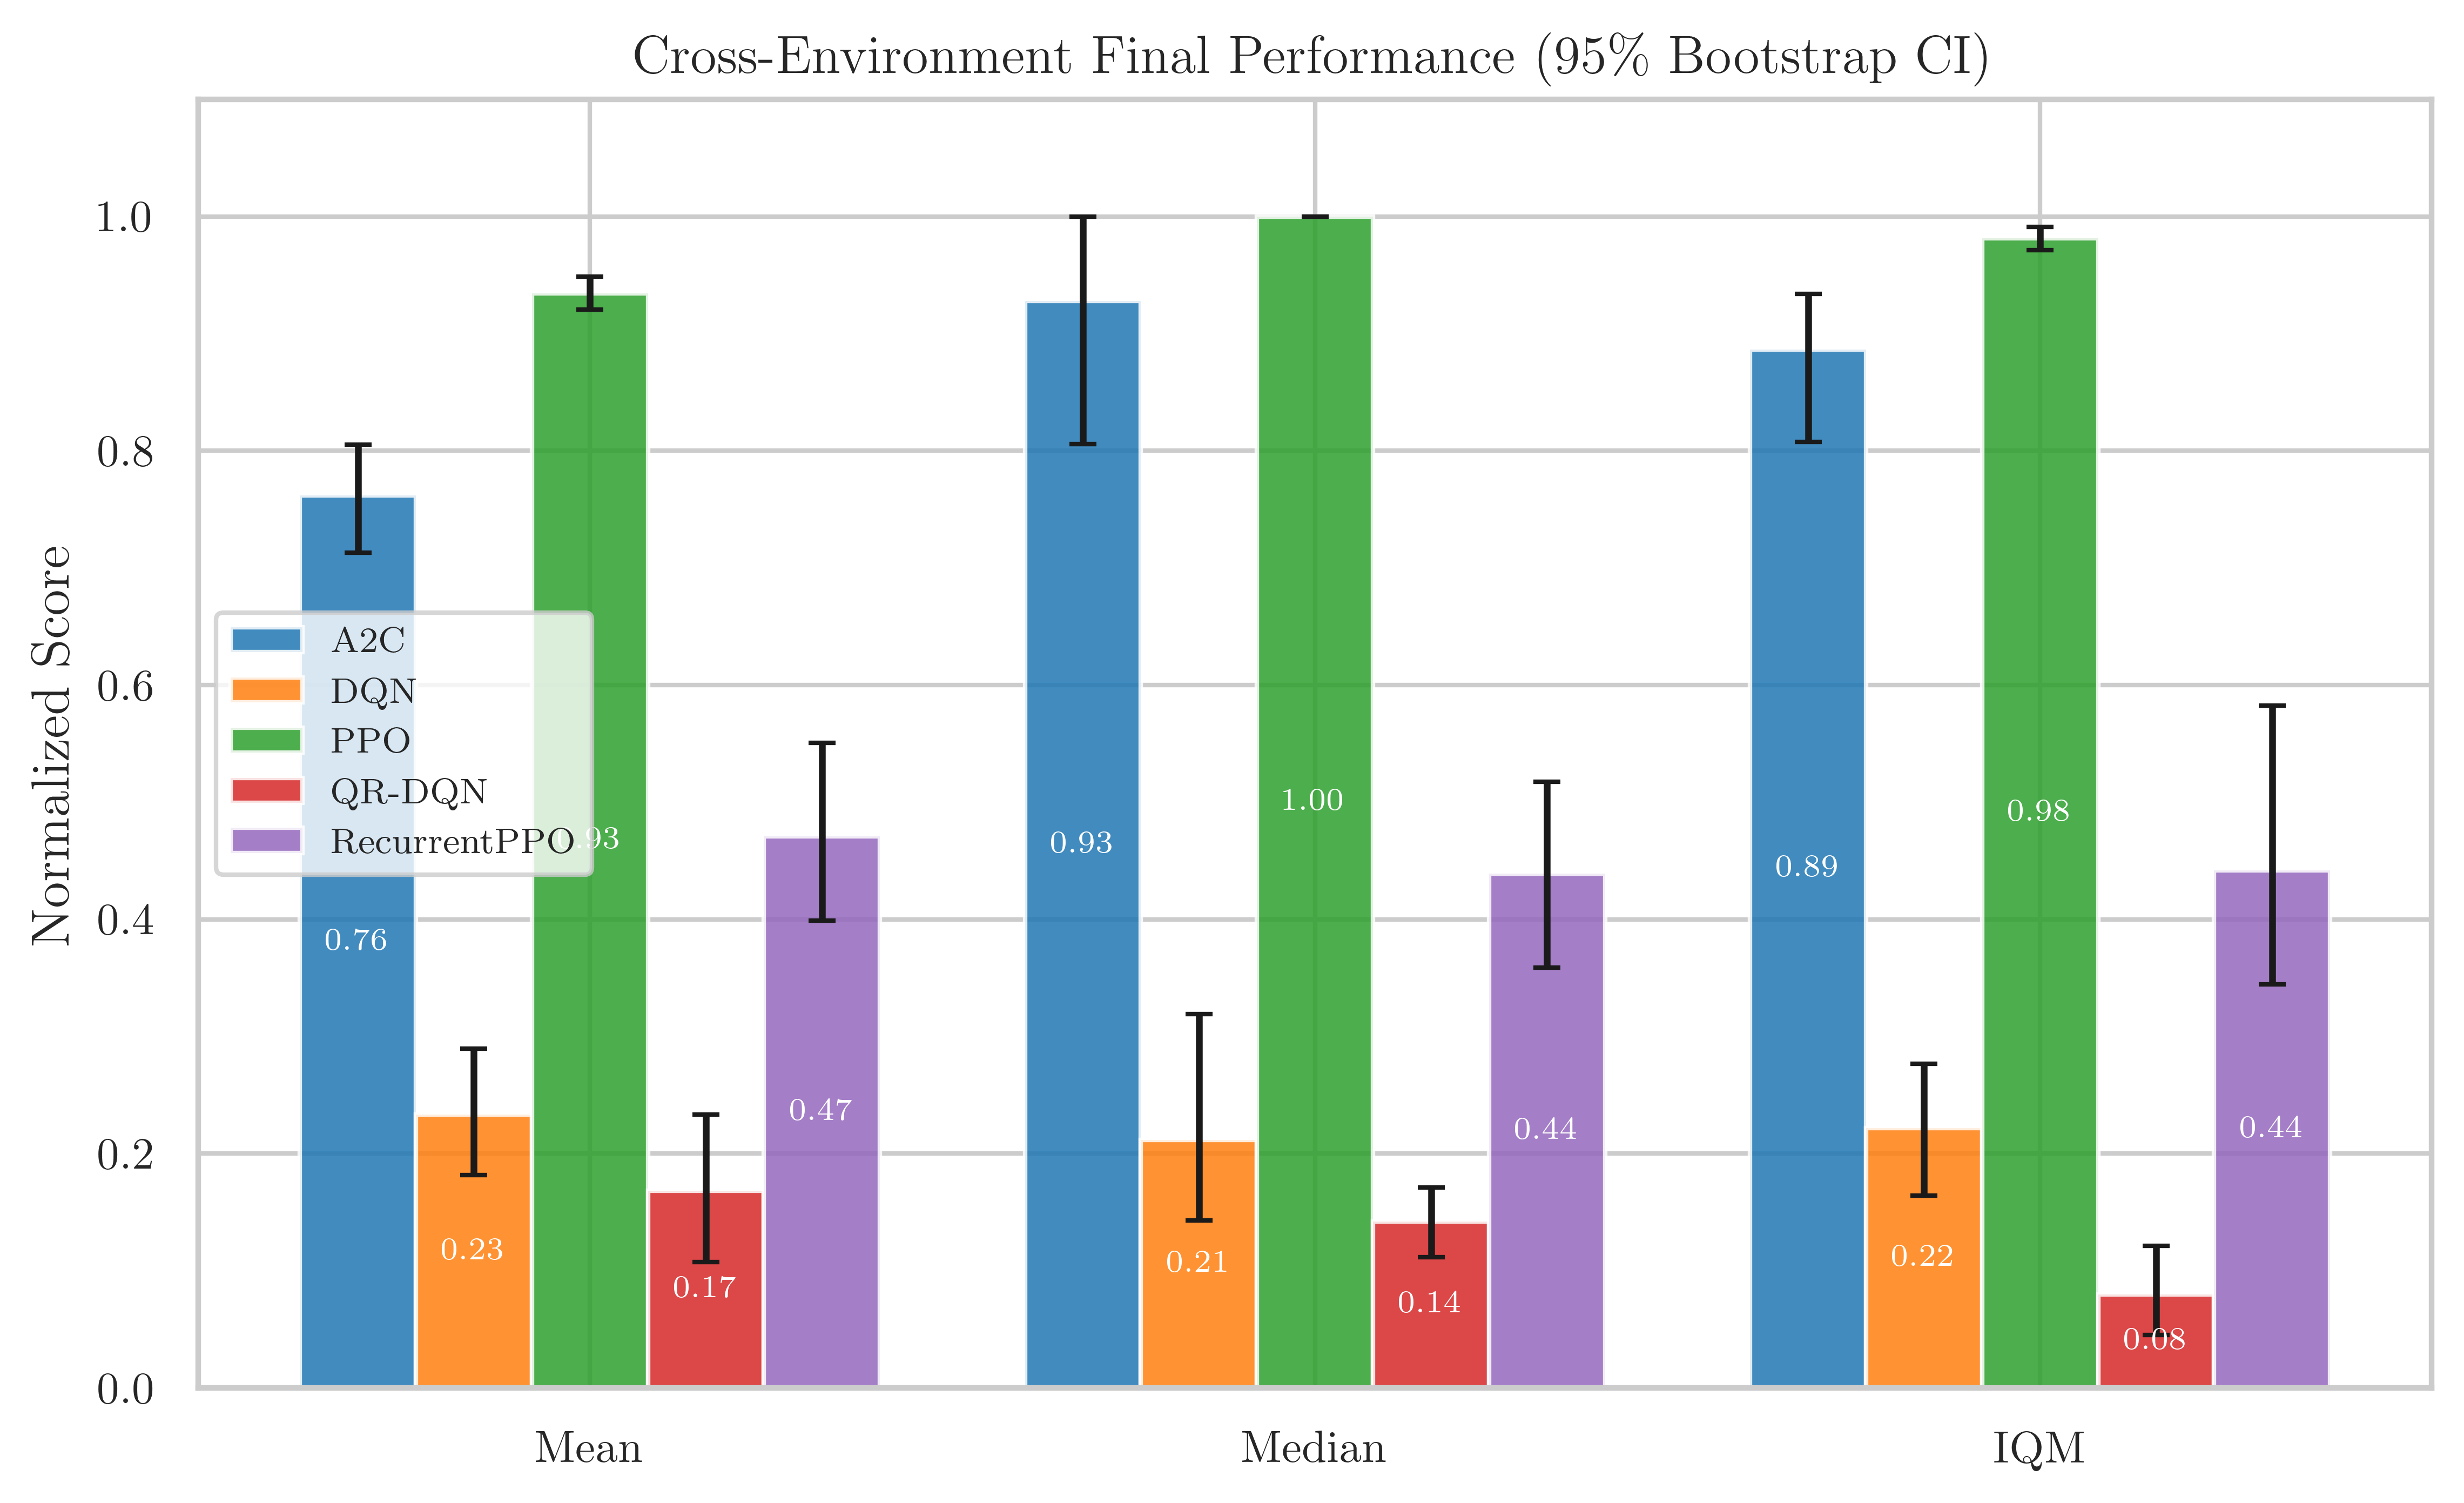
\includegraphics[width=\linewidth]{4_chapter/assets/final_performance.png}
  \caption{Cross-environment IQM, mean, and median with 95\% bootstrap
           confidence intervals.  PPO and A2C clearly separate from the
           remaining algorithms.}
  \label{fig:final-perf}
\end{figure}

\subsection{Performance Profile and Optimality Gap}
\label{sec:profile-gap}

The performance profile (Figure~\ref{fig:perf-profile}) shows the
fraction of runs exceeding normalised score $\tau$.  PPO maintains
$\hat{F}(\tau) > 0.9$ up to $\tau \approx 0.8$, whereas DQN and QR-DQN
drop below 50\% at $\tau = 0.3$.

\begin{figure}[ht]
  \centering
  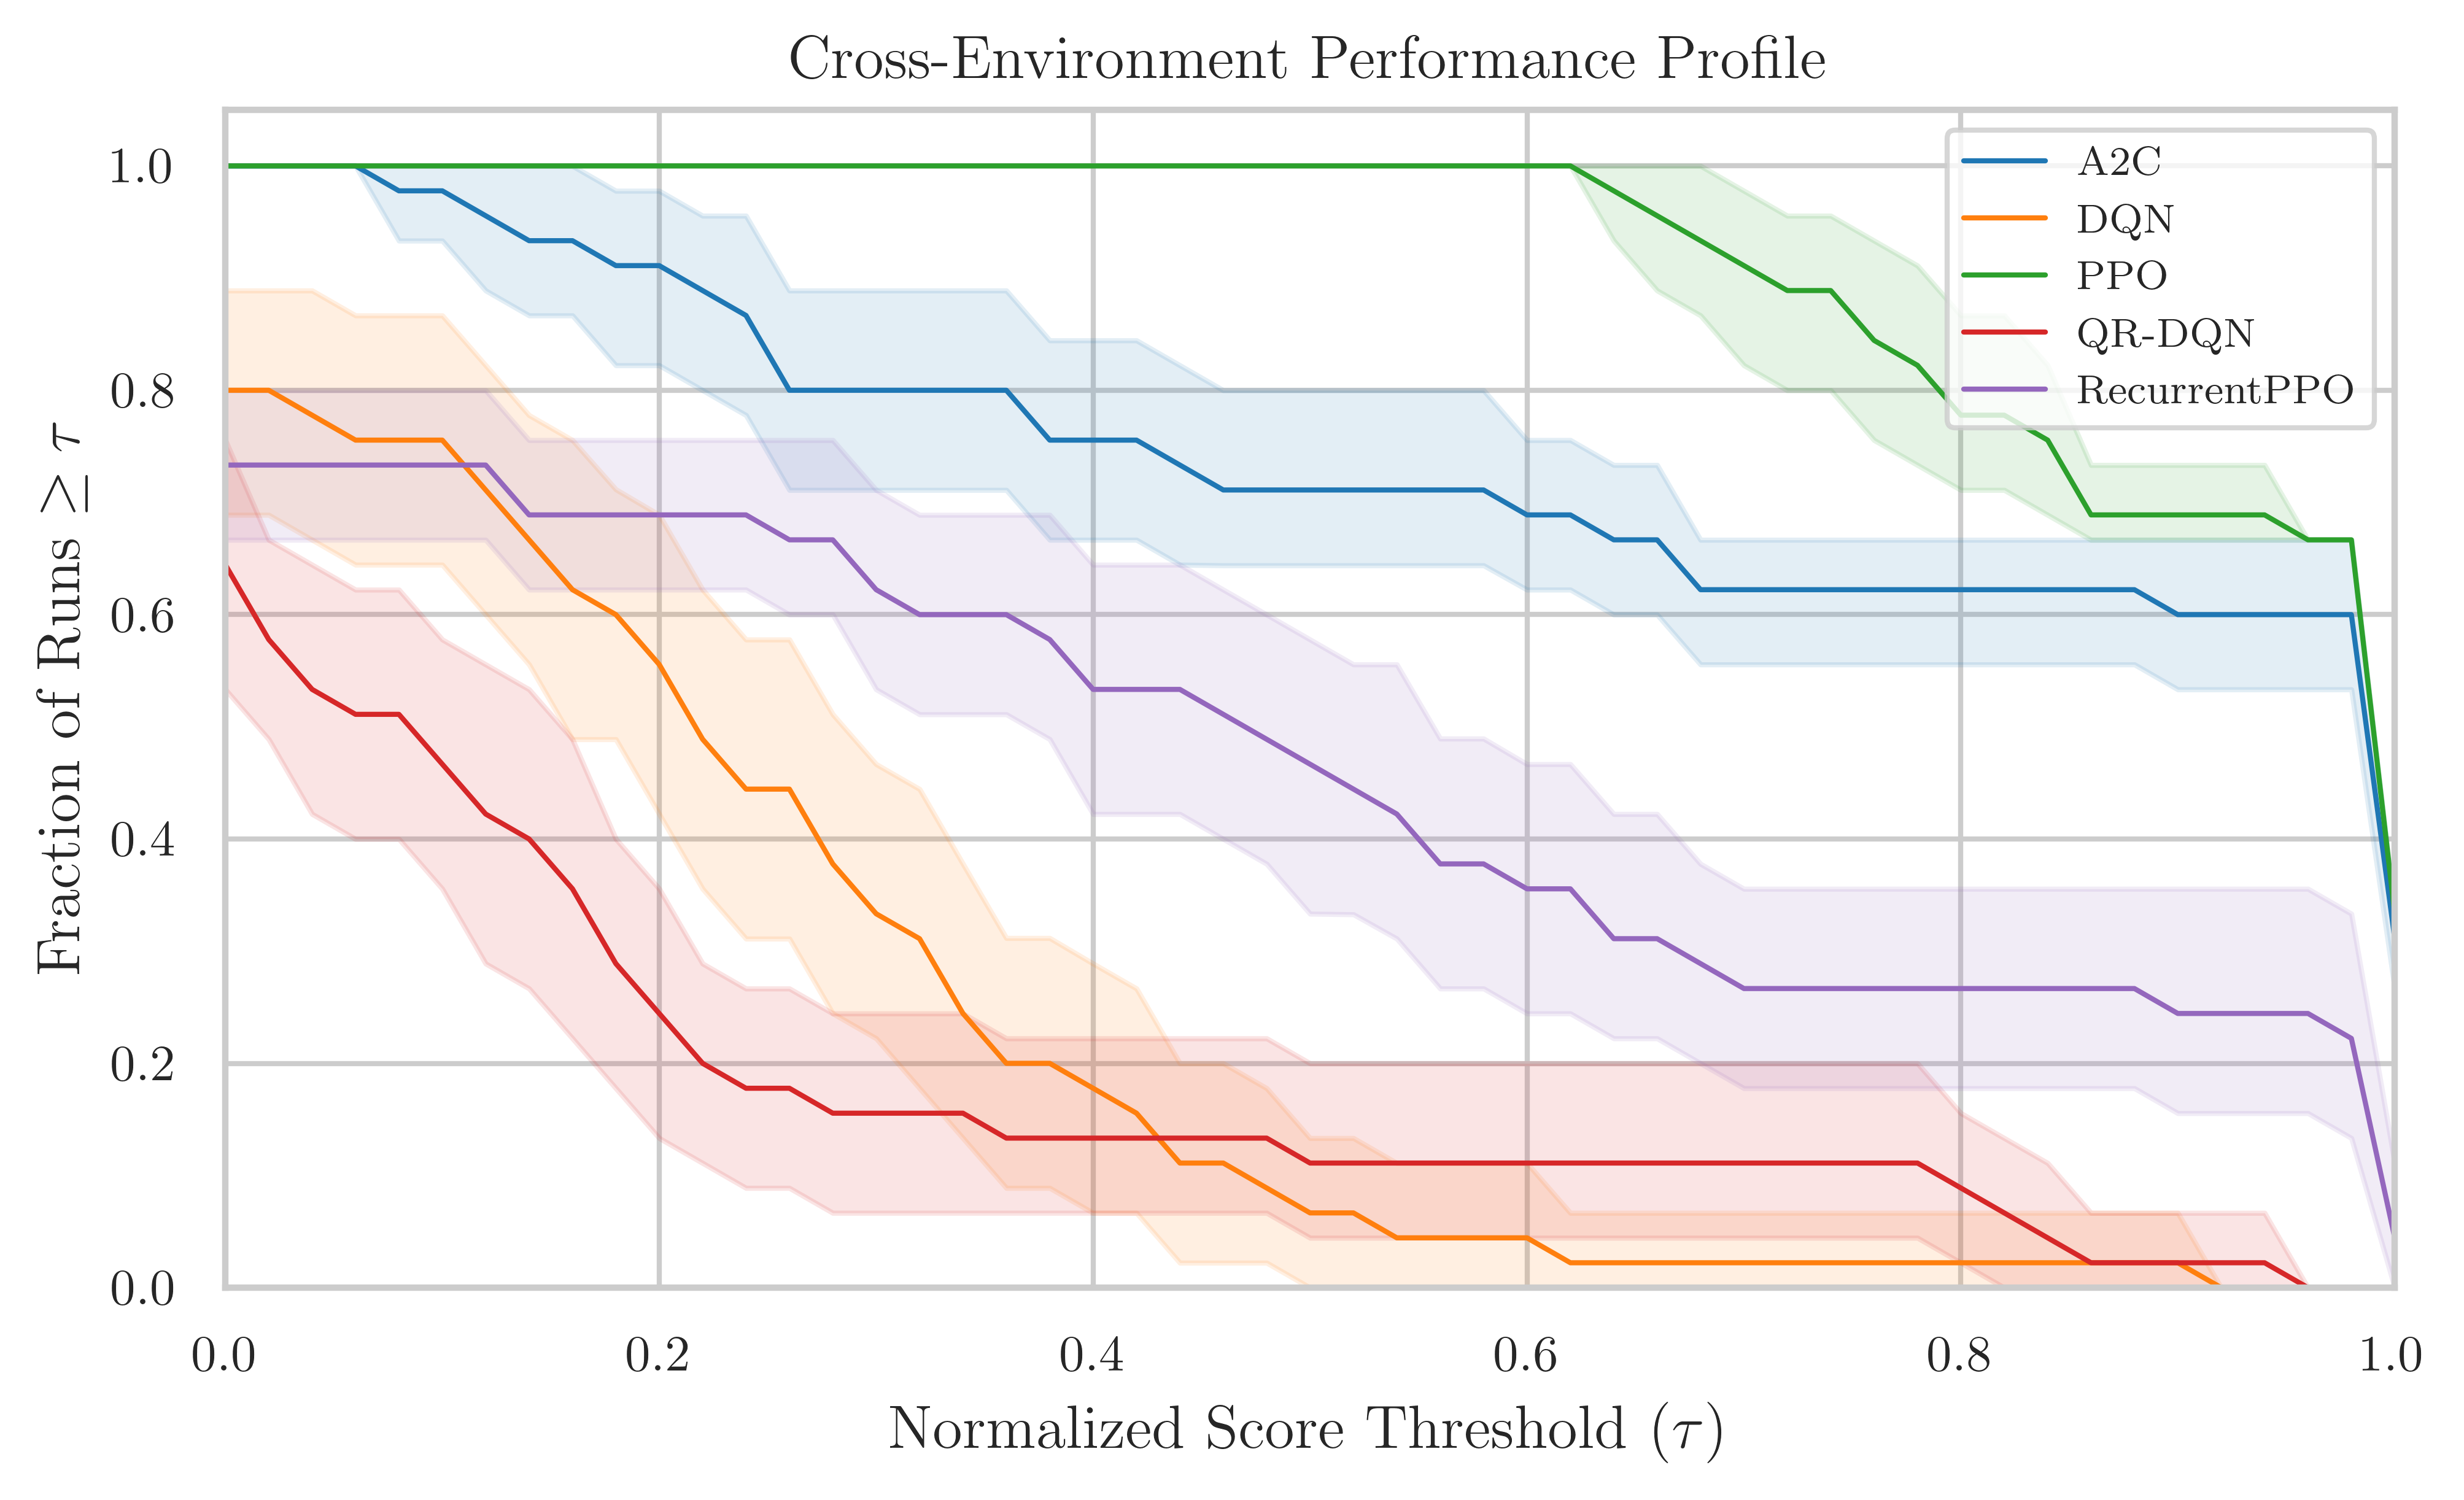
\includegraphics[width=\linewidth]{4_chapter/assets/performance_profile.png}
  \caption{Performance profiles with 95\% bootstrap CIs.  Higher curves
           indicate a larger fraction of runs exceeding each score
           threshold $\tau$.}
  \label{fig:perf-profile}
\end{figure}

\begin{figure}[ht]
  \centering
  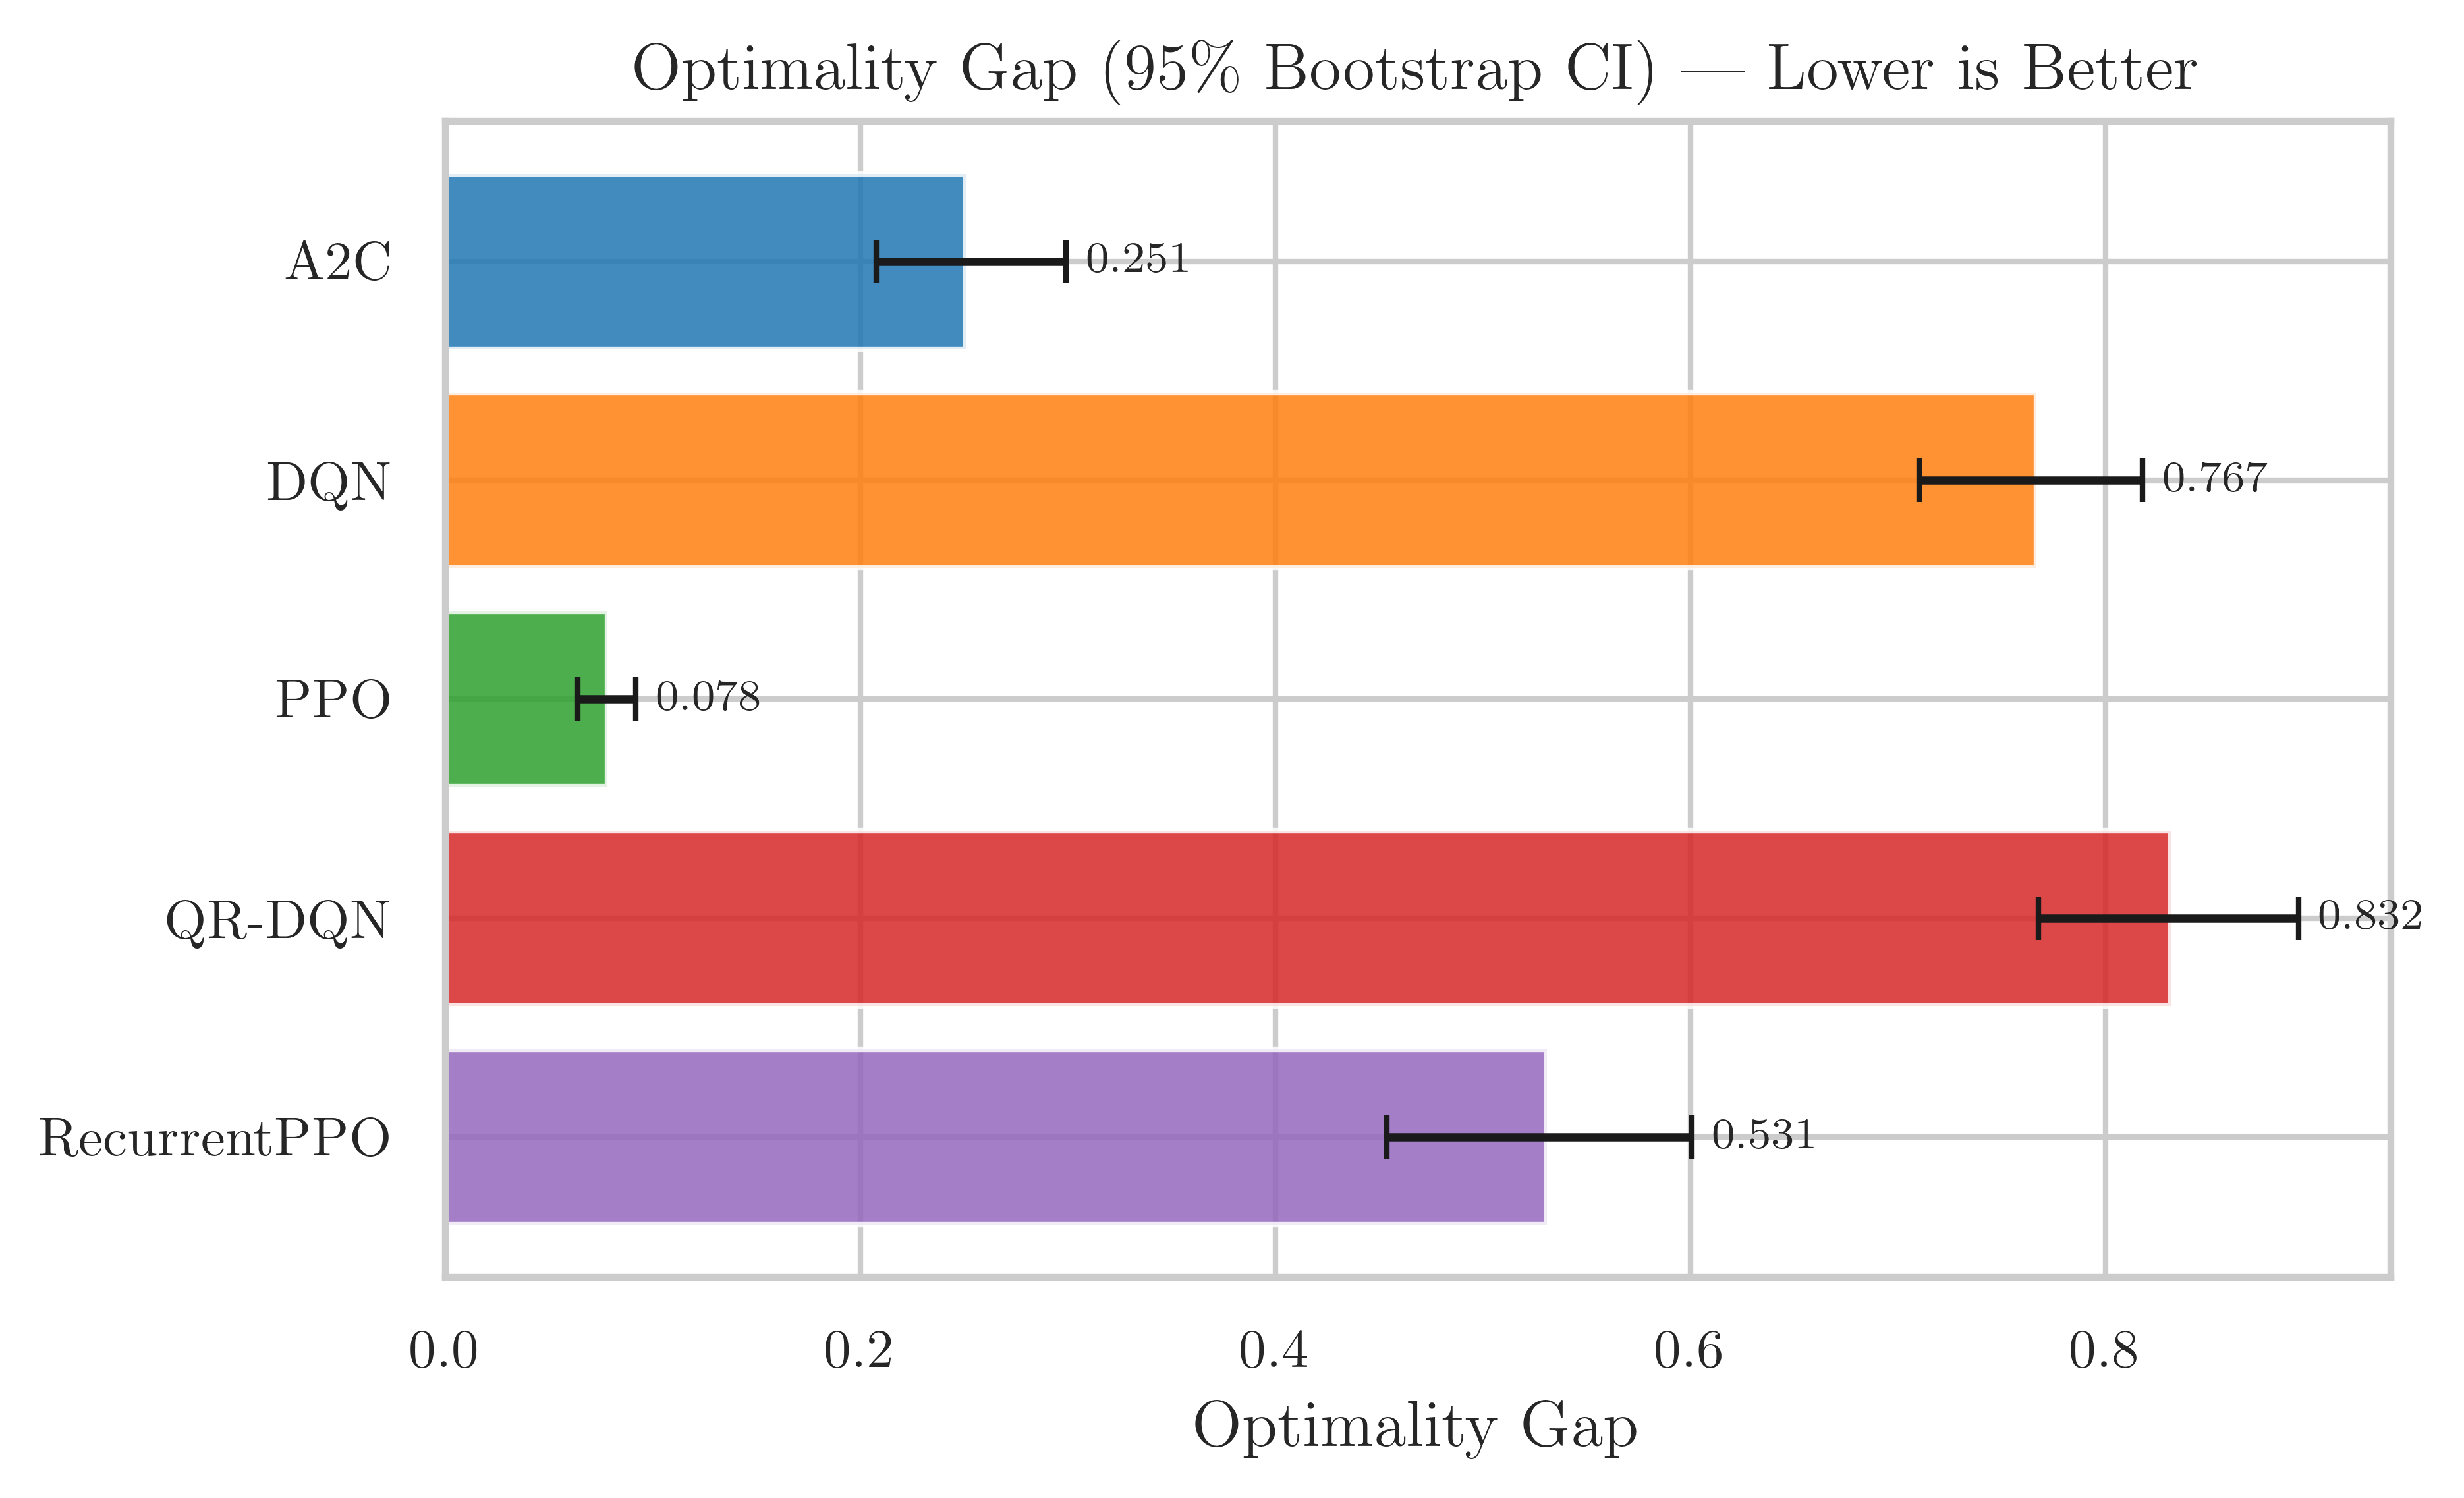
\includegraphics[width=\linewidth]{4_chapter/assets/optimality_gap.png}
  \caption{Optimality gap with 95\% bootstrap CIs.  Lower values indicate
           smaller shortfall from the target.  PPO ($0.078$) has the
           smallest gap; QR-DQN ($0.832$) has the largest.}
  \label{fig:opt-gap}
\end{figure}

\subsection{Sample Efficiency}
\label{sec:sample-eff}

Figures~\ref{fig:se-cartpole}--\ref{fig:se-combined} show sample
efficiency as normalised AUC over the training budget.

\begin{figure}[ht]
  \centering
  \begin{subfigure}[b]{0.48\linewidth}
    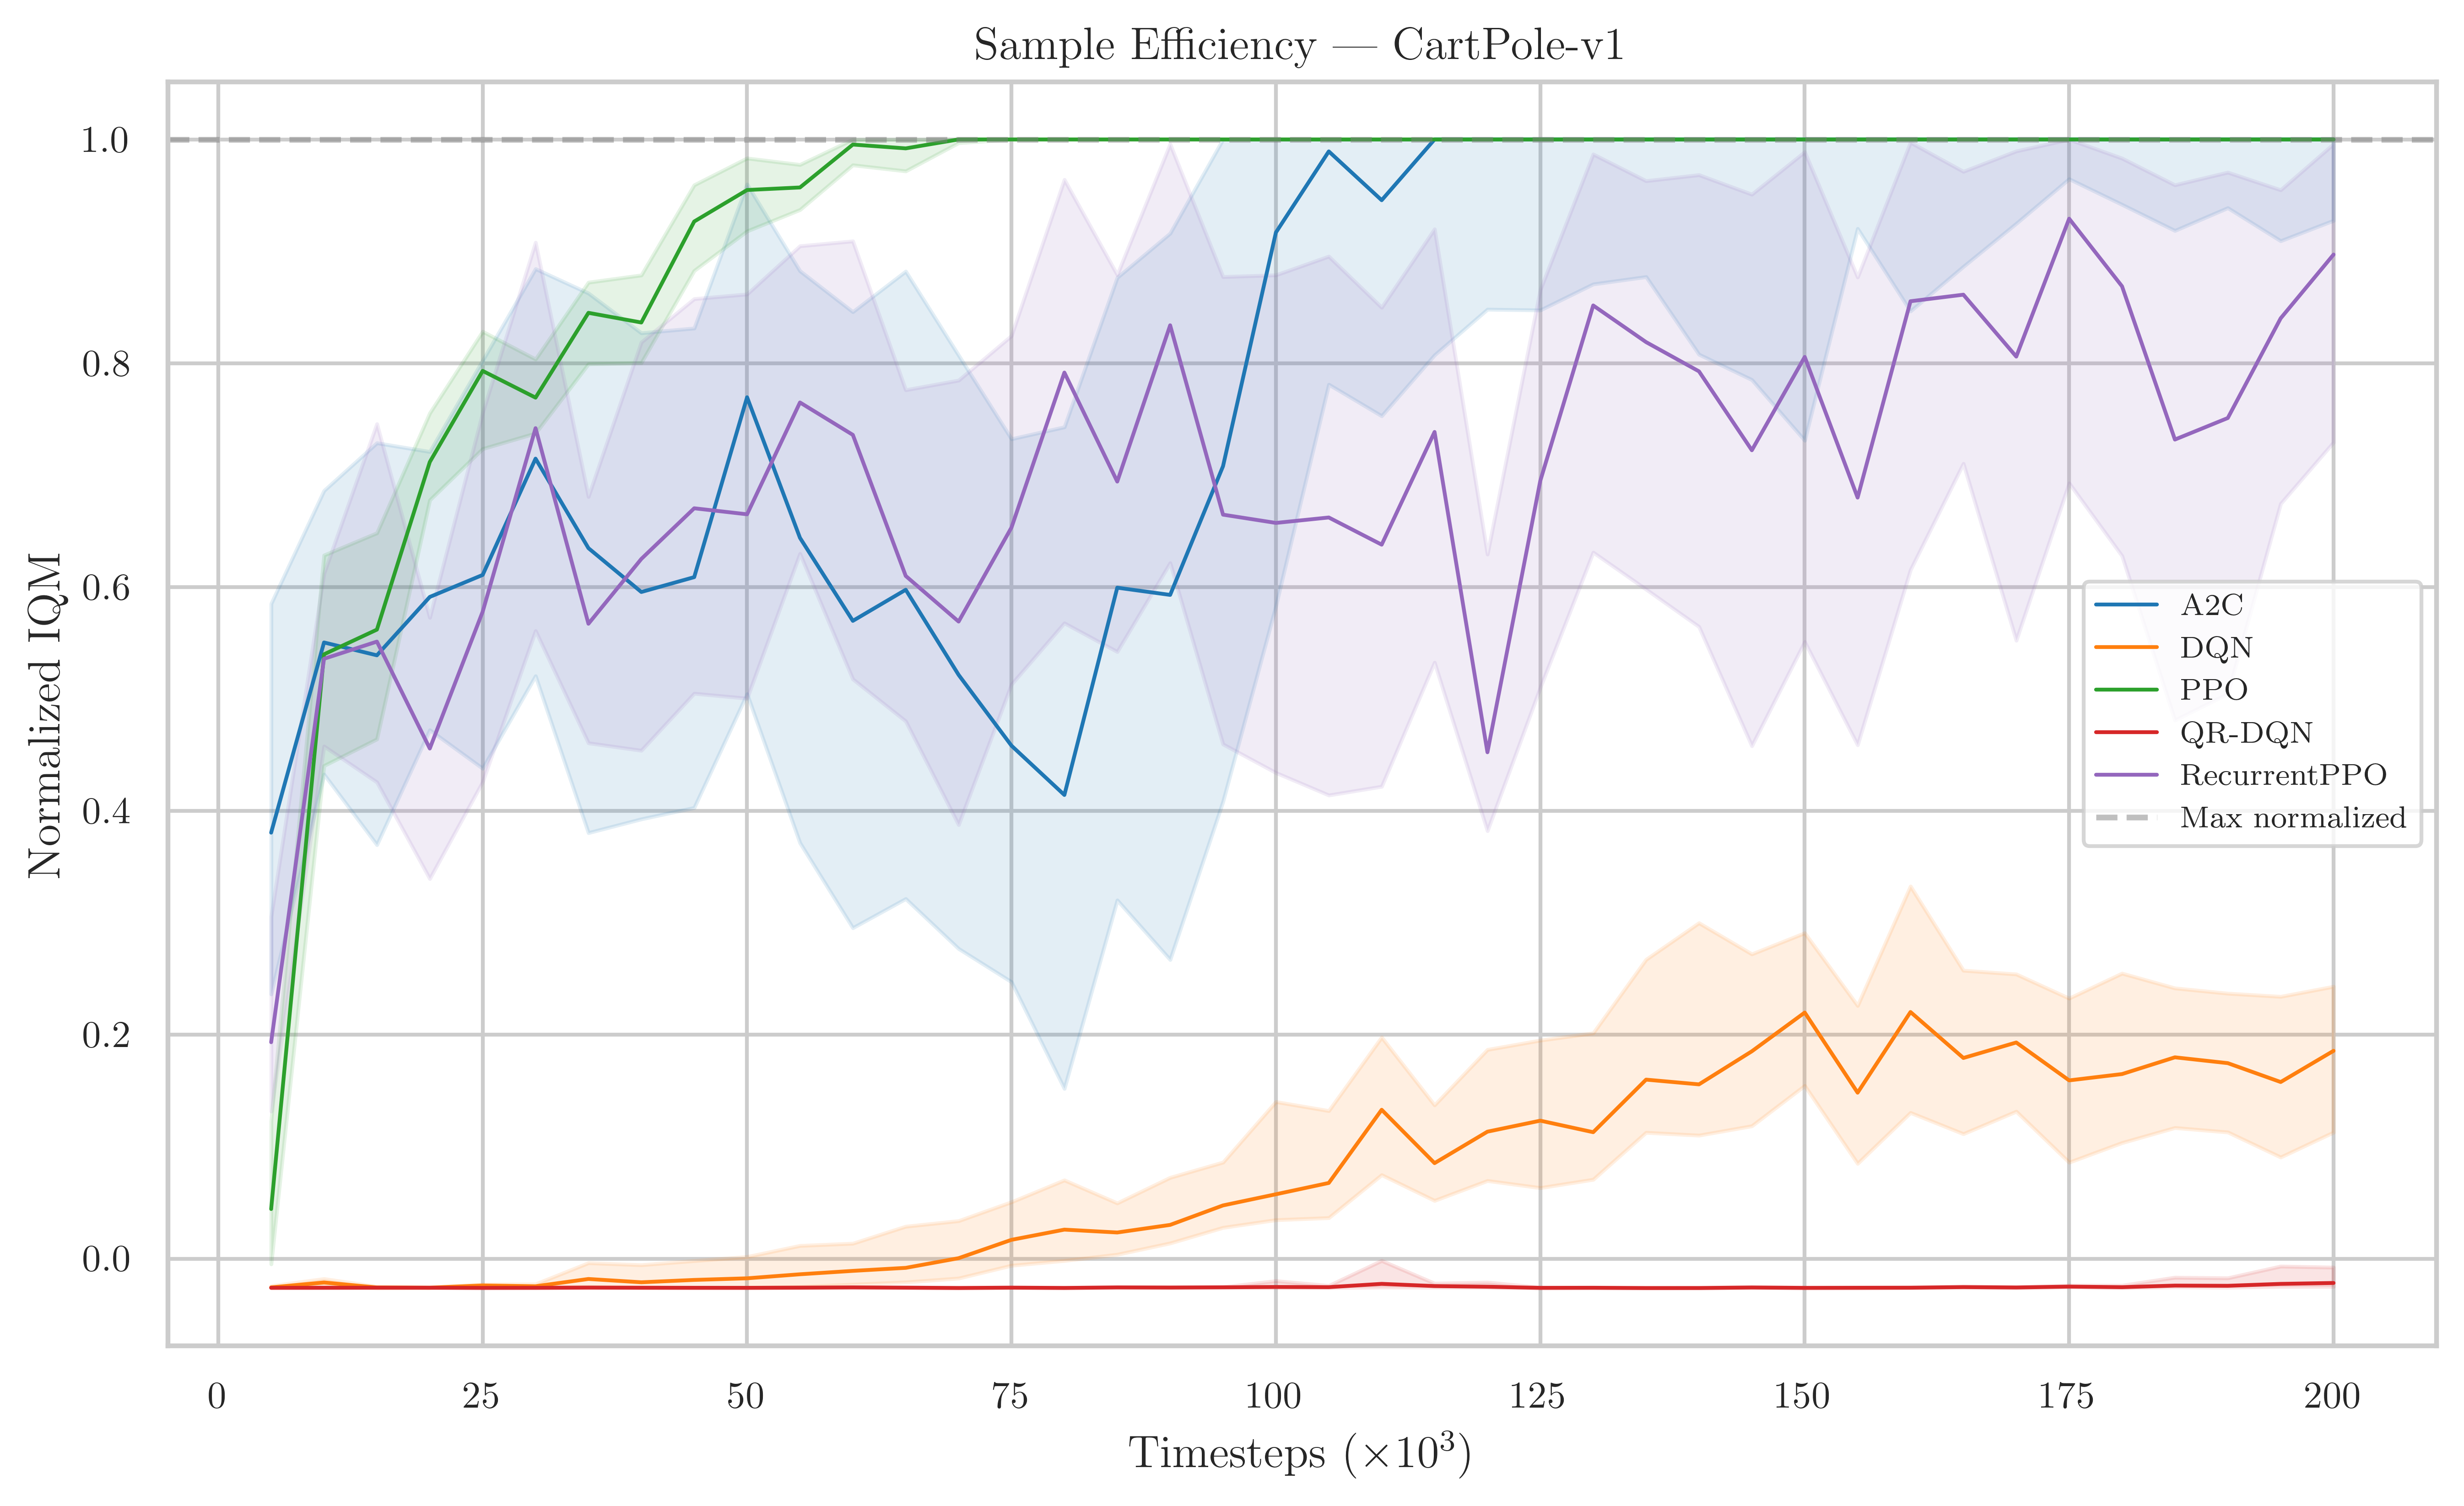
\includegraphics[width=\linewidth]{4_chapter/assets/sample_efficiency_cartpole-v1.png}
    \caption{CartPole-v1}
    \label{fig:se-cartpole}
  \end{subfigure}
  \hfill
  \begin{subfigure}[b]{0.48\linewidth}
    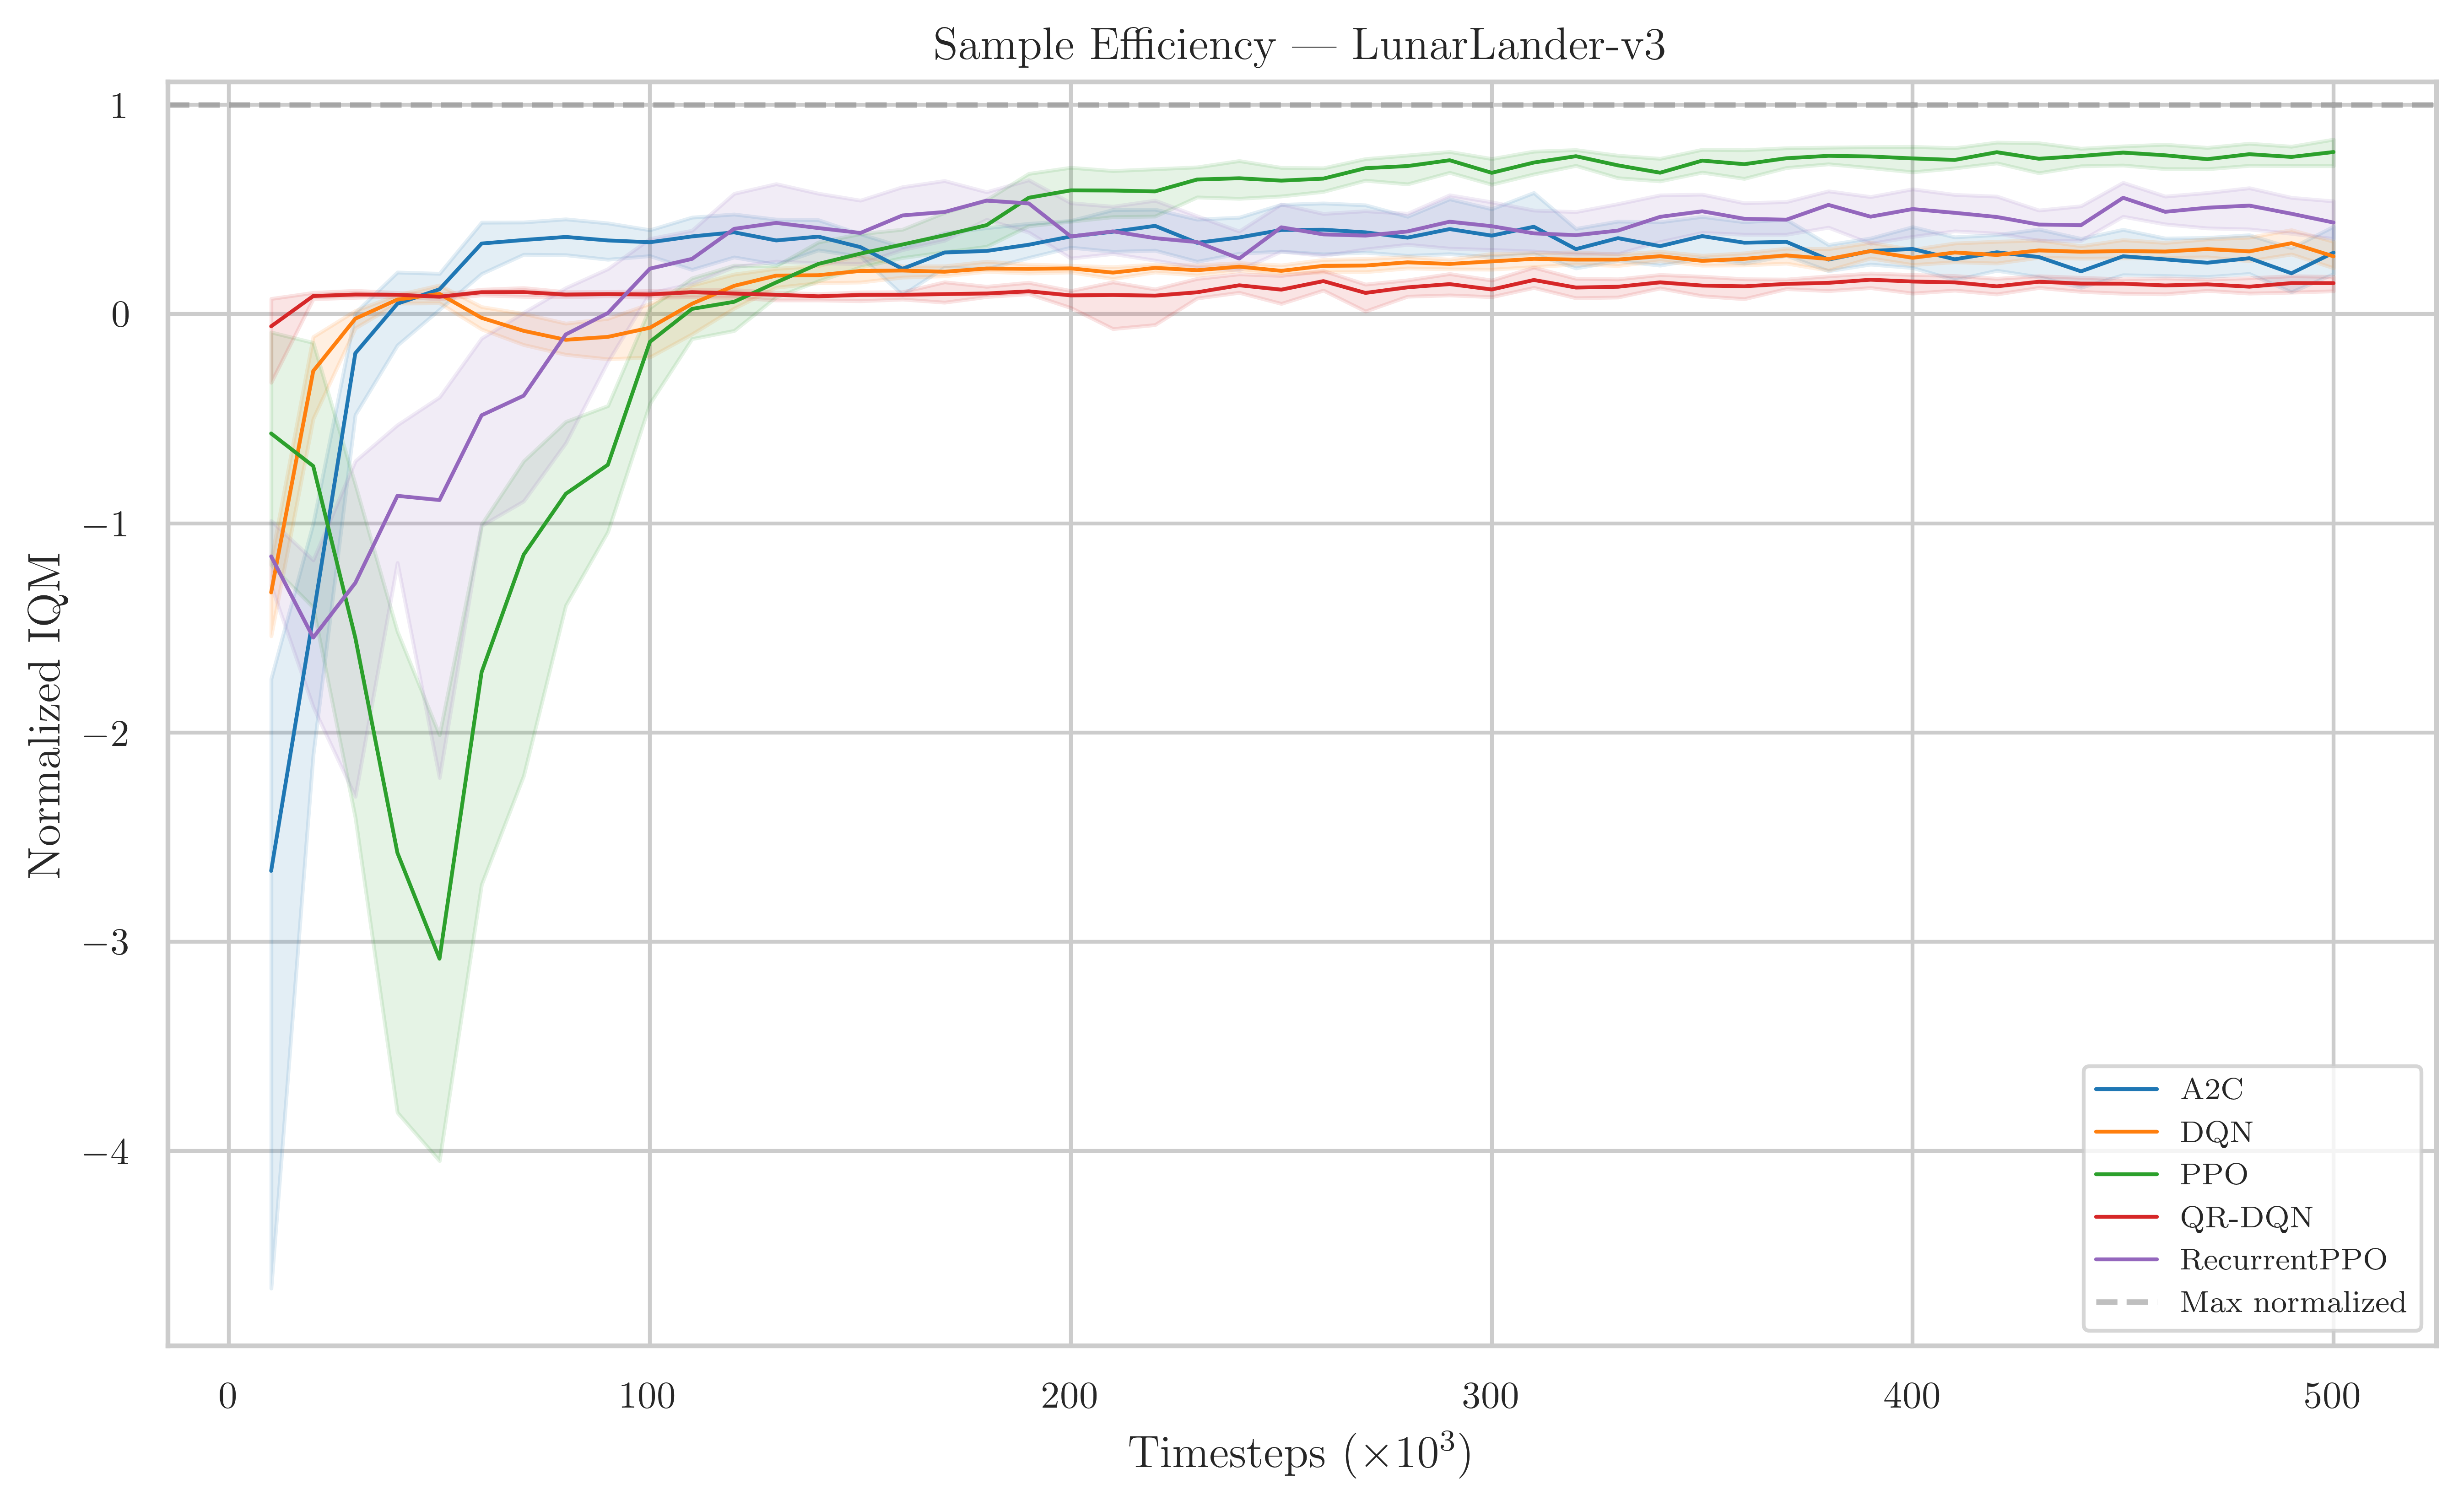
\includegraphics[width=\linewidth]{4_chapter/assets/sample_efficiency_lunarlander-v3.png}
    \caption{LunarLander-v3}
    \label{fig:se-lunarlander}
  \end{subfigure}

  \vspace{0.5em}
  \begin{subfigure}[b]{0.48\linewidth}
    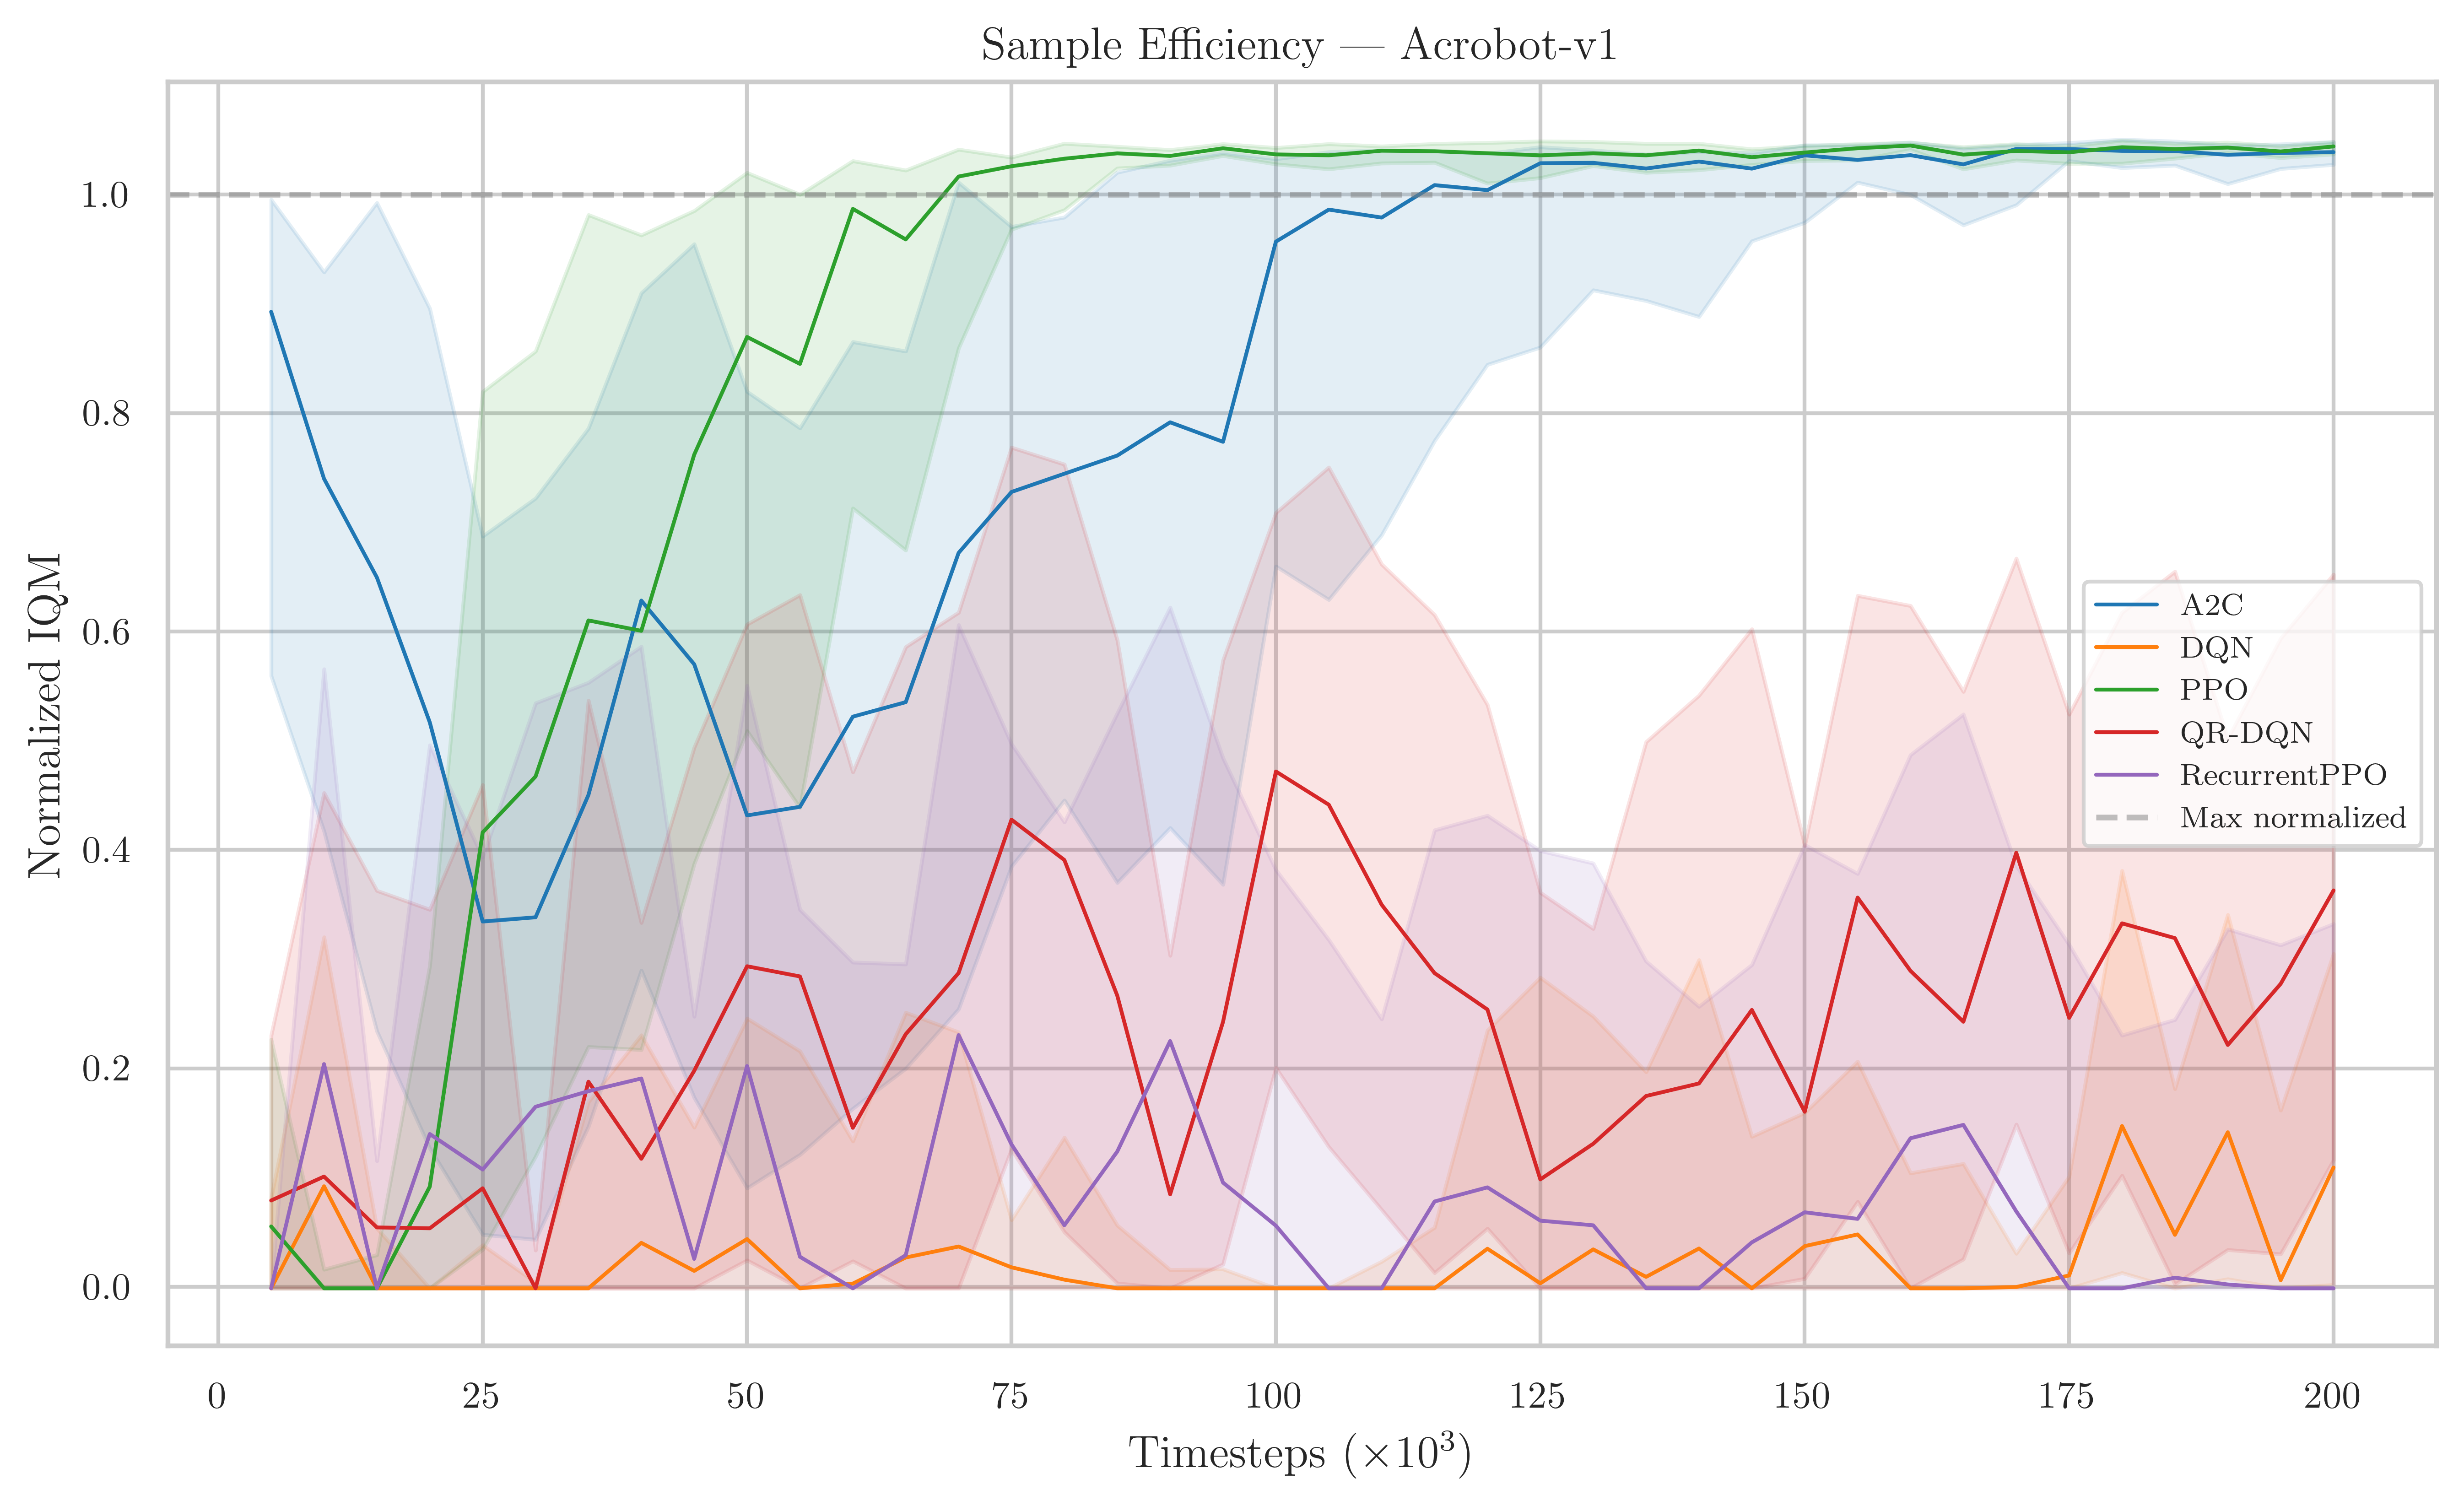
\includegraphics[width=\linewidth]{4_chapter/assets/sample_efficiency_acrobot-v1.png}
    \caption{Acrobot-v1}
    \label{fig:se-acrobot}
  \end{subfigure}
  \hfill
  \begin{subfigure}[b]{0.48\linewidth}
    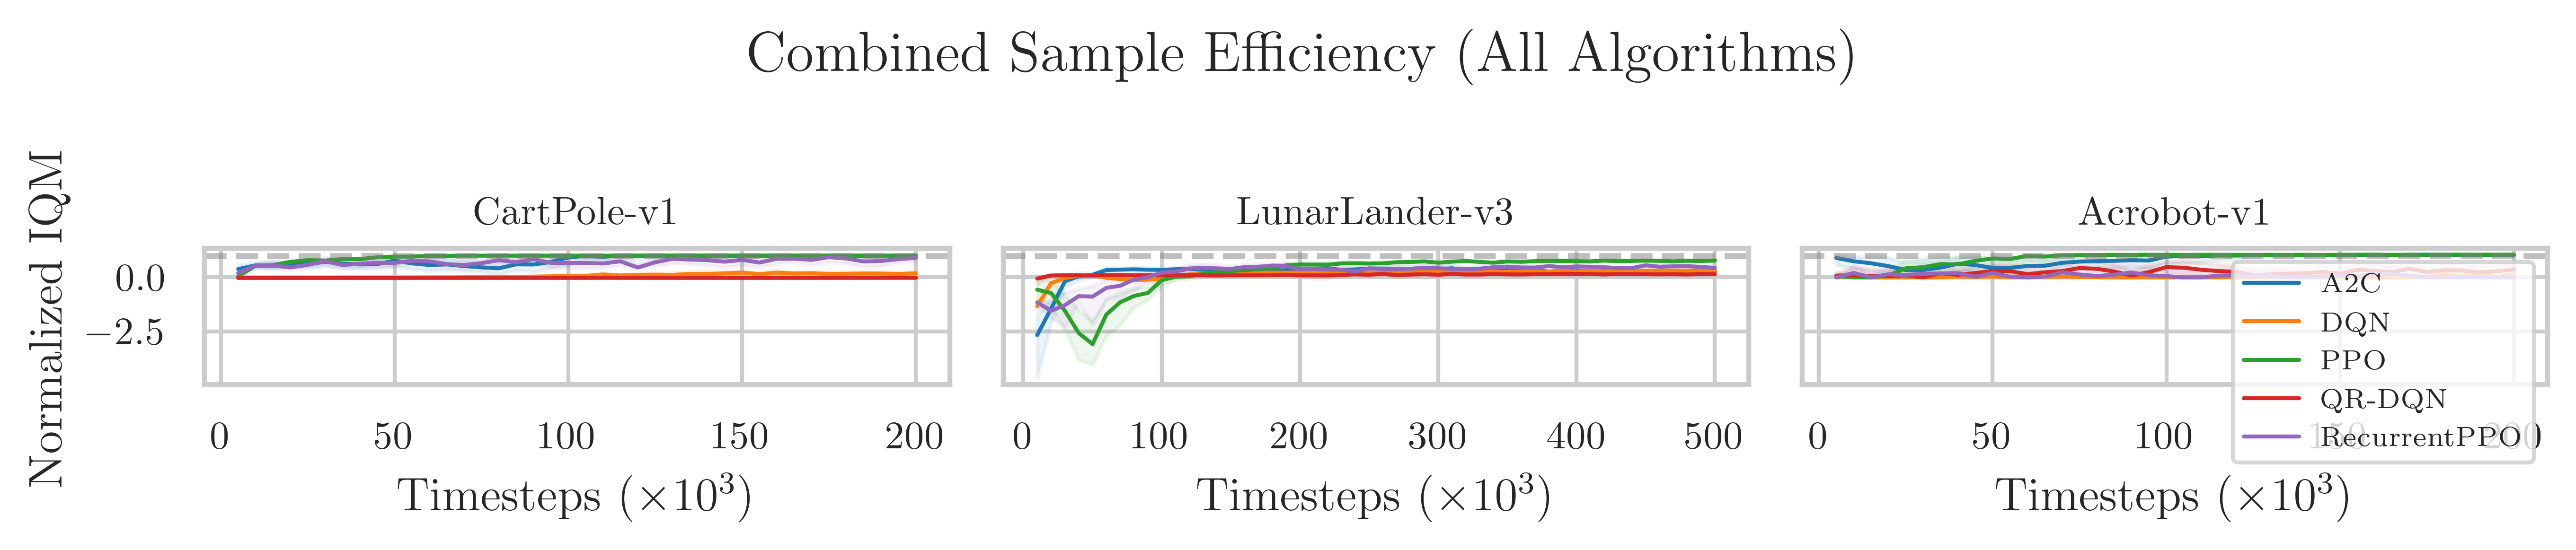
\includegraphics[width=\linewidth]{4_chapter/assets/combined_sample_efficiency.png}
    \caption{Combined (normalised)}
    \label{fig:se-combined}
  \end{subfigure}
  \caption{Sample efficiency (normalised AUC) per environment and combined.
           PPO and A2C lead on CartPole and Acrobot; all algorithms struggle
           on LunarLander.}
  \label{fig:sample-eff}
\end{figure}

Table~\ref{tab:sample-eff} reports the normalised AUC values.  PPO achieves
the highest sample efficiency on CartPole ($0.910$) and Acrobot ($0.853$).
On LunarLander, all algorithms achieve similar AUC ($0.17$--$0.24$),
reflecting the difficulty of this environment.

\begin{table}[ht]
\centering
\caption{Sample efficiency (normalised AUC) per environment.}
\label{tab:sample-eff}
\begin{tabular}{lccc}
\toprule
\textbf{Algorithm} & \textbf{CartPole-v1} & \textbf{LunarLander-v3}
                   & \textbf{Acrobot-v1} \\
\midrule
PPO    & 0.910 & 0.226 & 0.853 \\
A2C    & 0.782 & 0.238 & 0.801 \\
RPPO   & 0.685 & 0.225 & 0.075 \\
DQN    & 0.075 & 0.169 & 0.022 \\
QR-DQN & $-0.025$ & 0.115 & 0.229 \\
\bottomrule
\end{tabular}
\end{table}

\subsection{Pairwise Probability of Improvement}
\label{sec:poi}

Table~\ref{tab:poi} and Figure~\ref{fig:poi} report the pairwise probability of improvement $P(A > B)$, averaged across environments. PPO has $P > 0.89$ against every other algorithm.


\begin{table}[ht]
\centering
\caption{Pairwise probability of improvement $P(\text{row} > \text{col})$,
         averaged across environments.}
\label{tab:poi}
\begin{tabular}{lccccc}
\toprule
         & \textbf{PPO} & \textbf{A2C} & \textbf{RPPO}
         & \textbf{DQN} & \textbf{QR-DQN} \\
\midrule
PPO    & ---   & 0.656 & 0.896 & 1.000 & 1.000 \\
A2C    & 0.344 & ---   & 0.642 & 0.830 & 0.939 \\
RPPO   & 0.104 & 0.358 & ---   & 0.692 & 0.744 \\
DQN    & 0.000 & 0.170 & 0.308 & ---   & 0.721 \\
QR-DQN & 0.000 & 0.061 & 0.256 & 0.279 & ---   \\
\bottomrule
\end{tabular}
\end{table}

\begin{figure}[ht]
  \centering
  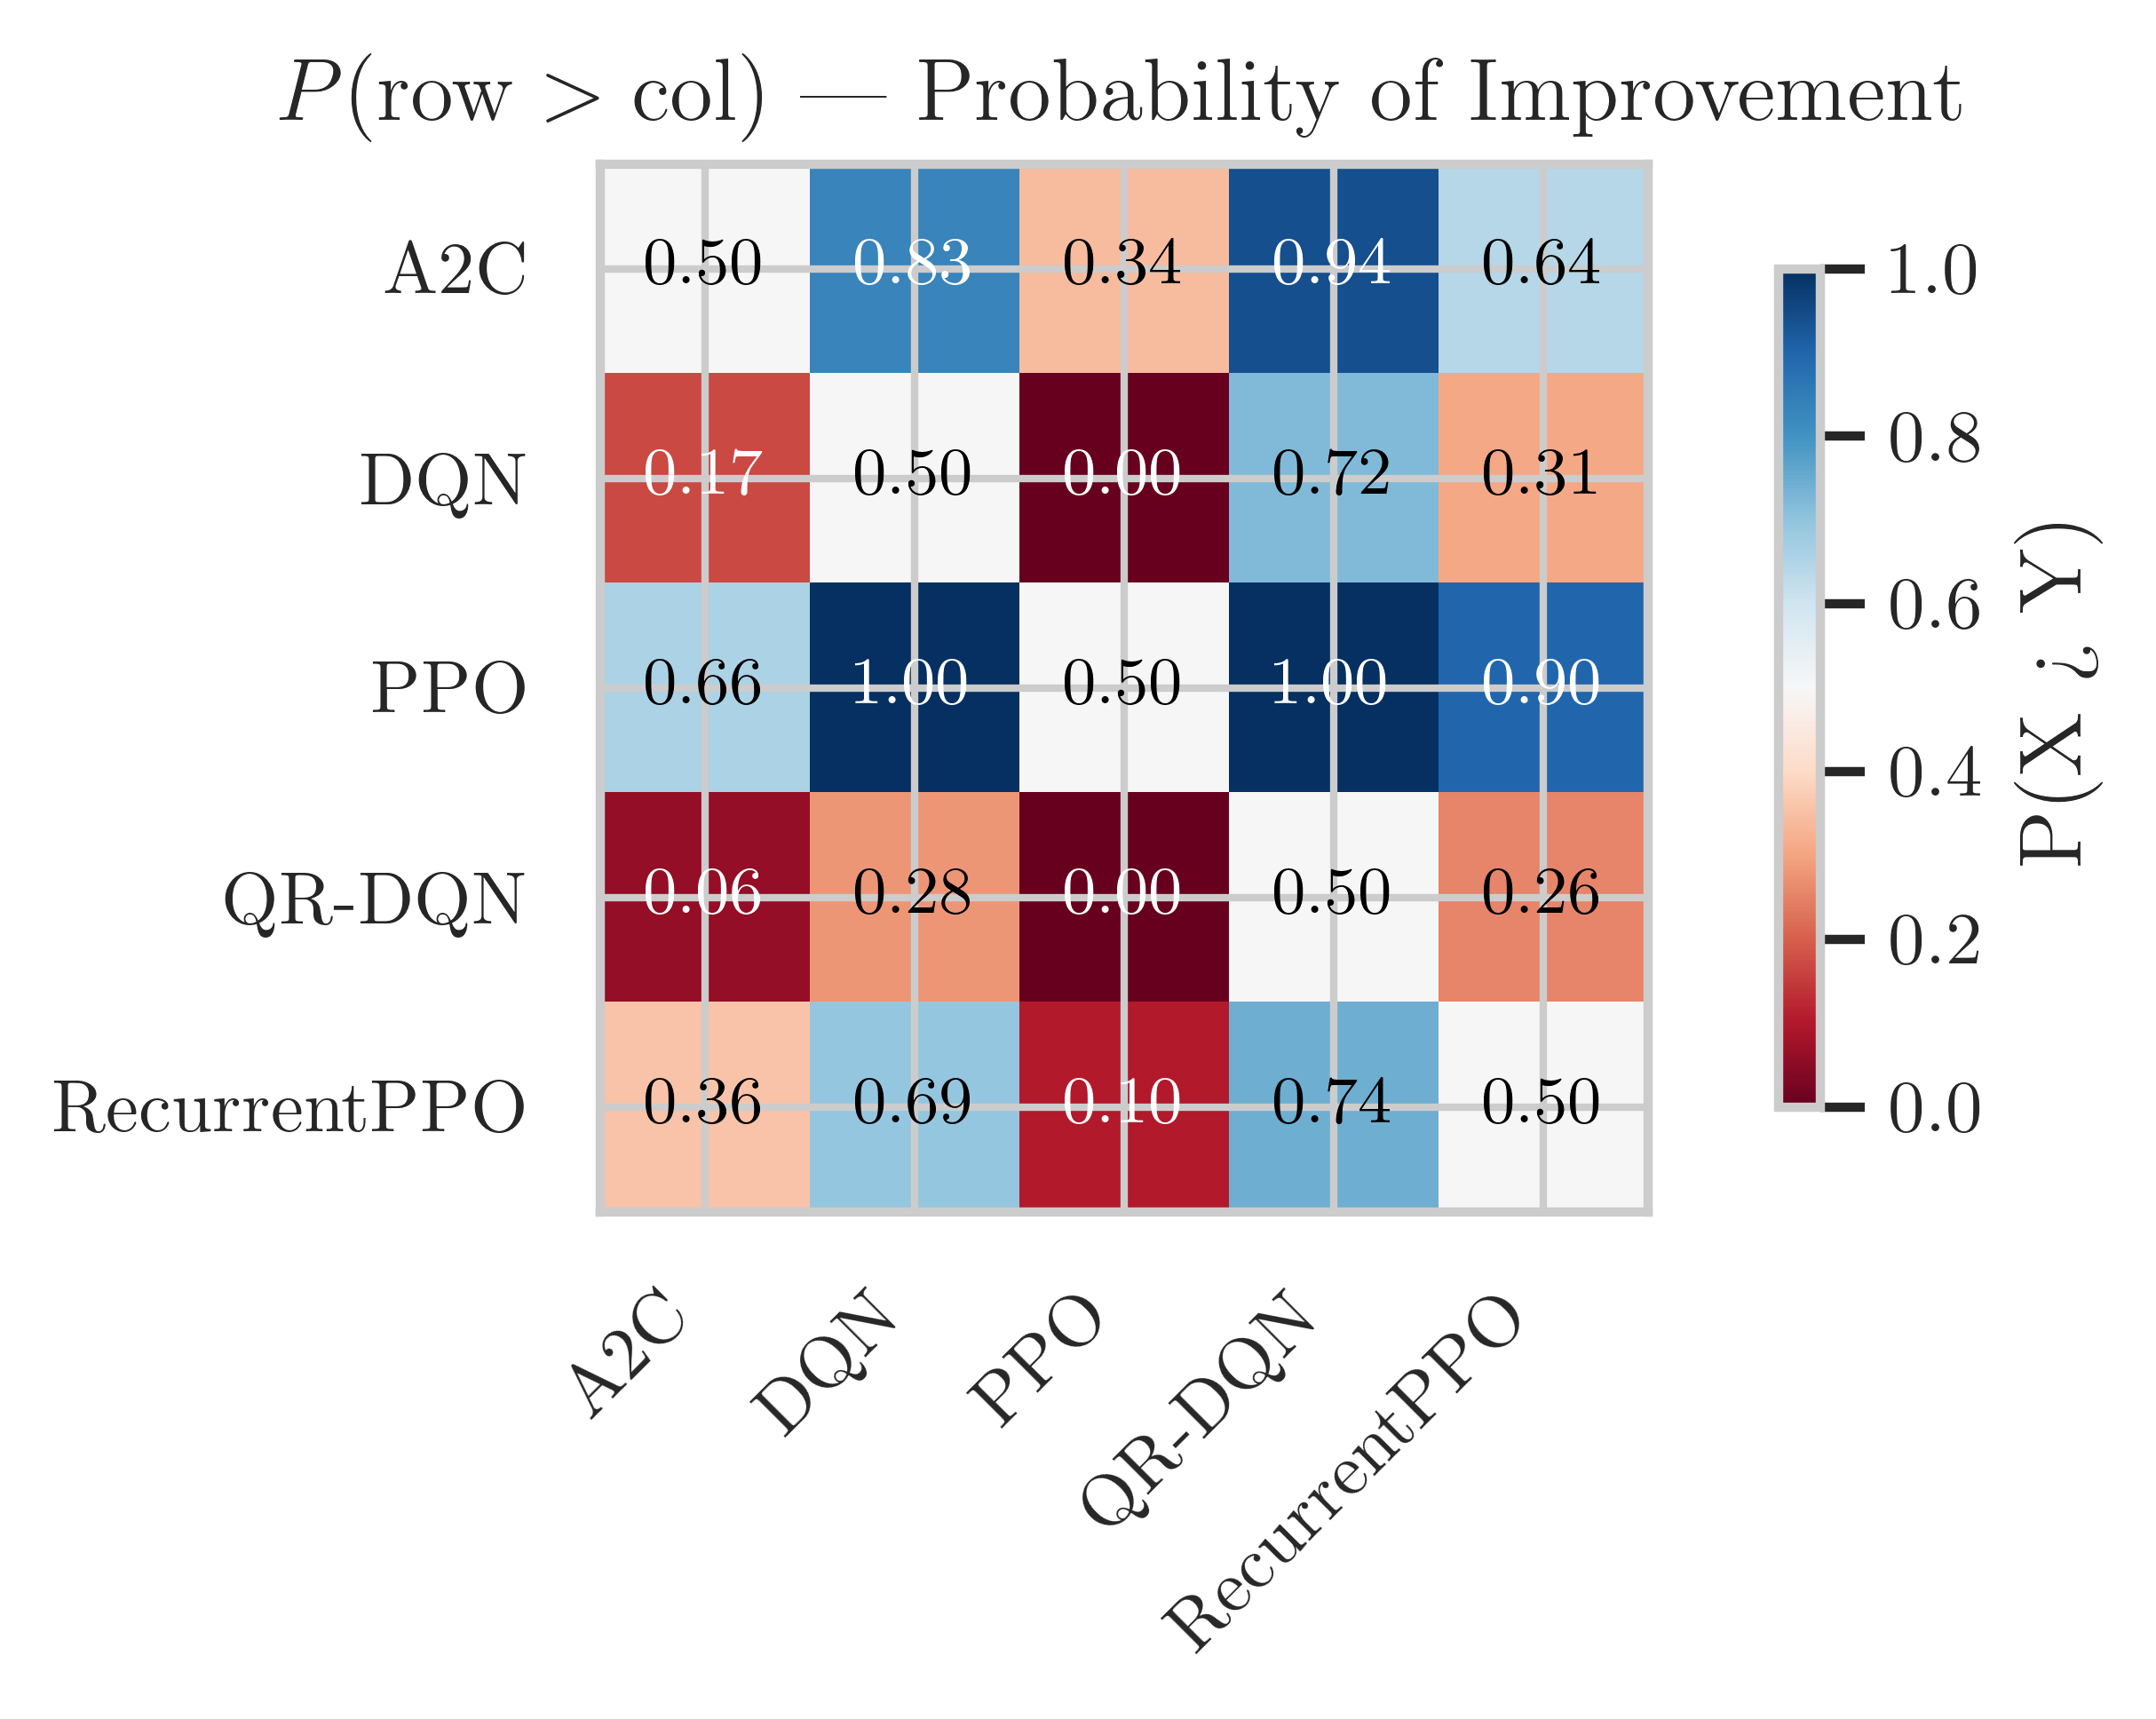
\includegraphics[width=0.8\linewidth]{4_chapter/assets/poi_heatmap.png}
  \caption{Probability-of-improvement heatmap.  PPO dominates all pairwise
           comparisons.  DQN vs QR-DQN is the closest pairing ($0.721$).}
  \label{fig:poi}
\end{figure}

\subsection{Wall-Clock Timing Analysis}
\label{sec:timing}

\begin{figure}[ht]
  \centering
  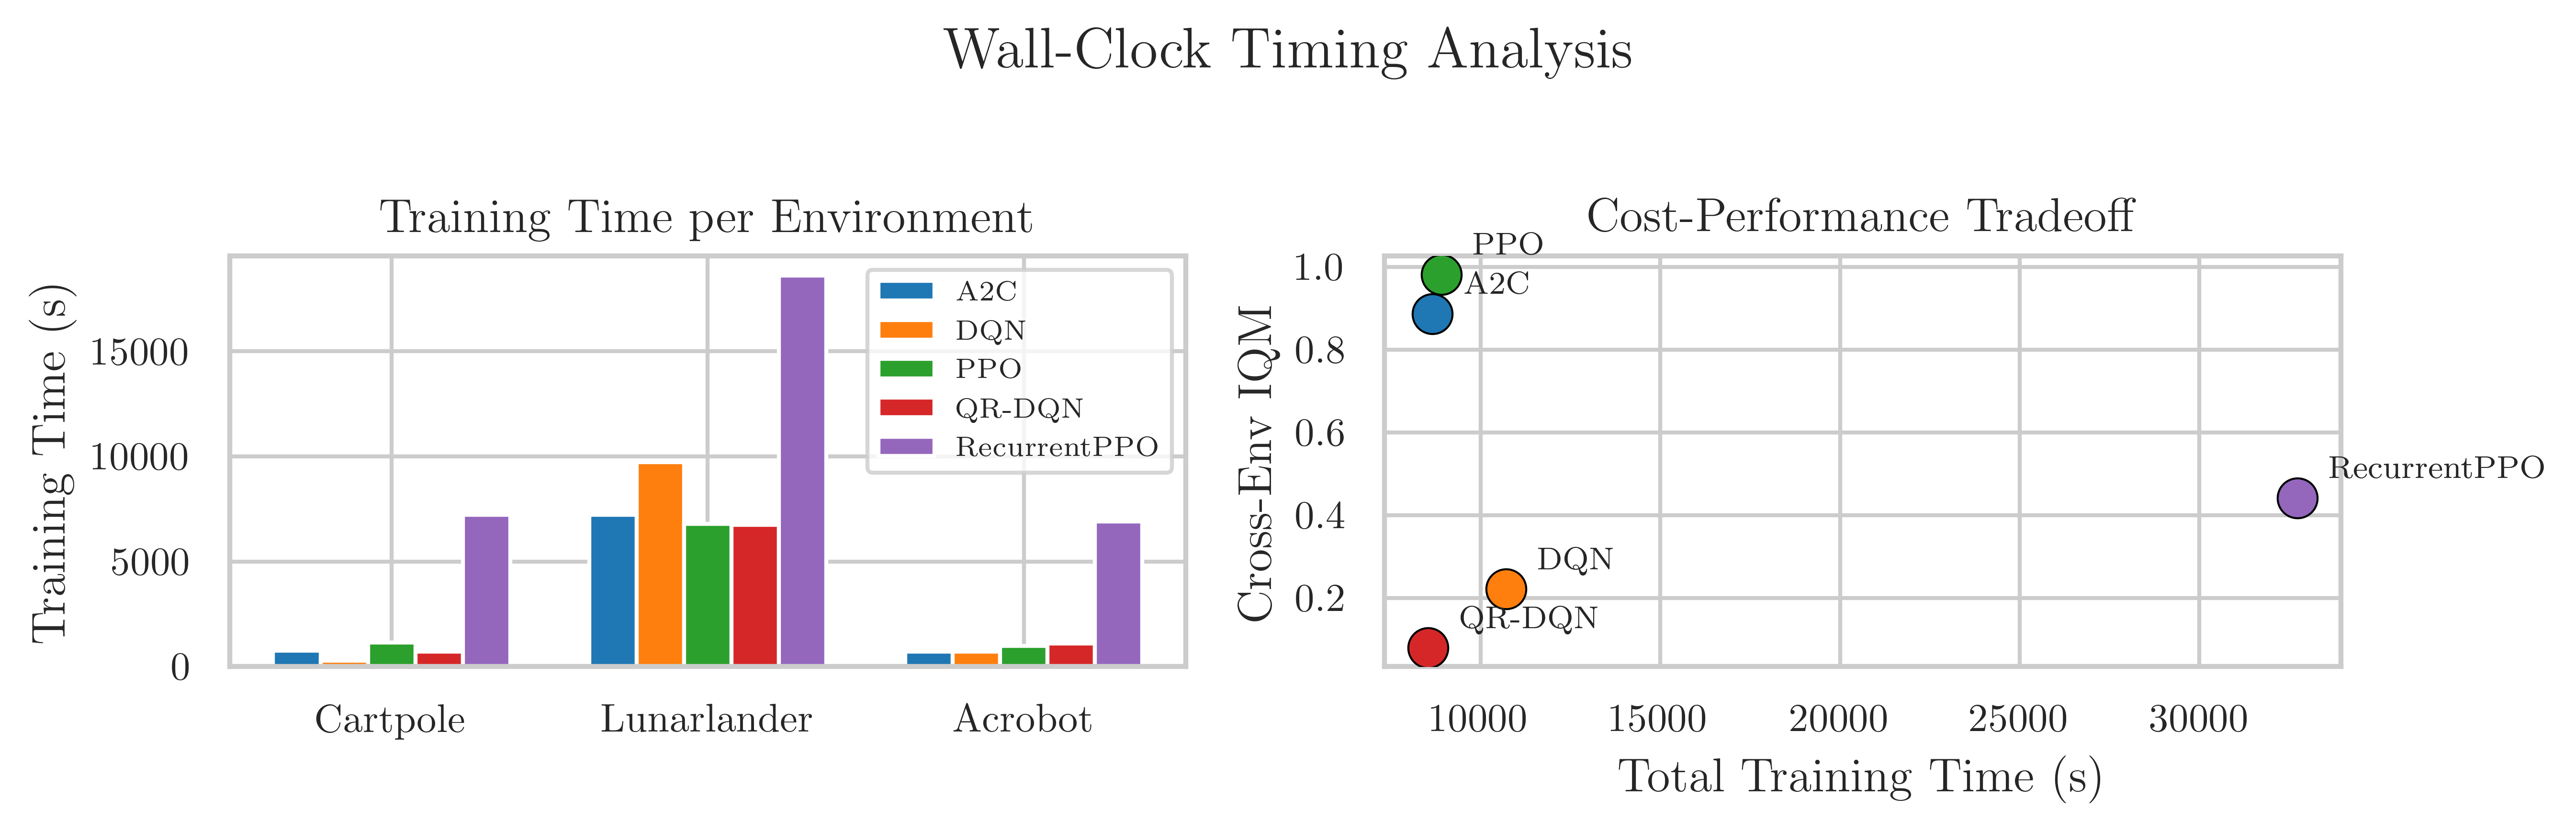
\includegraphics[width=\linewidth]{4_chapter/assets/timing_analysis.png}
  \caption{Wall-clock training time per algorithm and environment.  RPPO
           is $3$--$4\times$ slower than all other algorithms due to the
           recurrent architecture.}
  \label{fig:timing}
\end{figure}

%% ------------------------------------------------------------------
\section{Key Findings}
\label{sec:key-findings}

\begin{enumerate}

\item \textbf{PPO is the dominant algorithm.}
      It ranks first on every aggregate metric (IQM $0.981$, optimality gap
      $0.078$) and achieves $P(\text{PPO} > X) \ge 0.656$ against every
      competitor.  On CartPole it achieves zero-variance convergence to the
      maximum return; on Acrobot it slightly exceeds the theoretical maximum.
      Its only relative weakness is LunarLander, where it still leads
      (IQM $0.768$) but with moderate variance across seeds.

\item \textbf{A2C is the runner-up with high variance.}
      A2C matches PPO on CartPole and Acrobot (IQM $\ge 1.0$) but
      underperforms on LunarLander (IQM $0.303$), where its IQR of
      $120.9$ raw-reward units reveals high sensitivity to the random seed.
      Cross-environment IQM ($0.886$) is substantially below PPO ($0.981$),
      and the pairwise probability of A2C beating PPO is only $0.344$.

\item \textbf{RPPO is inappropriate for fully-observed MDPs.}
      Despite using the same PPO objective, the LSTM policy is $3.5\times$
      slower to train and fails catastrophically on Acrobot
      (IQM $-0.001$), where 12 of 15 seeds remain at the random-policy
      floor.  On LunarLander it outperforms A2C (IQM $0.444$ vs.\ $0.303$),
      suggesting that the recurrence provides a small advantage on tasks with
      longer temporal dependencies.  However, its overall ranking (IQM
      $0.442$, optimality gap $0.531$) makes it a poor default choice.

\item \textbf{DQN and QR-DQN are sample-starved.}
      Both DQN-family algorithms fail under the given training budgets,
      especially on CartPole and Acrobot (200K steps).
      DQN achieves cross-environment IQM $0.222$; QR-DQN is worse at
      $0.080$.  QR-DQN's distributional value head adds representational
      capacity but requires more data to learn effectively than standard DQN.
      Their off-policy nature, combined with the replay-buffer warm-up phase
      and $\varepsilon$-greedy exploration, requires substantially more
      samples to converge compared to on-policy methods on these
      low-dimensional environments.

\end{enumerate}

%% ------------------------------------------------------------------
\section{Discussion}
\label{sec:discussion}

\paragraph{Methodological notes.}
The metrics section described two per-environment metrics that were not
computed in the final evaluation pipeline: \emph{success rate} (omitted
because none of the three environments define a binary success condition)
and \emph{CVaR} tail-risk (computed but not visualised separately, as the
per-seed heatmap and box-swarm plots already expose seed-level failures).
All other metrics---learning curves, final IQM with bootstrap CIs,
sample efficiency AUC, performance profiles, optimality gap, and pairwise
probability of improvement---were computed exactly as defined.

\paragraph{Limitations.}
Several limitations constrain the generalisability of these results:
\begin{itemize}
  \item \textbf{Small environment suite ($M = 3$).}  Cross-environment
        aggregates describe only these three tasks and should not be
        interpreted as general claims about algorithm families
        \citep{agarwal2021precipice, patterson2024edrl}.
  \item \textbf{Default hyperparameters.}  No per-algorithm tuning was
        performed.  DQN and QR-DQN may benefit significantly from adjusted
        learning rates, replay buffer sizes, or longer training budgets.
  \item \textbf{Fixed training budget.}  The budgets (200K--500K steps)
        may be insufficient for off-policy algorithms that require a
        warm-up phase.  A fairer comparison would either extend the budget
        or include a wall-clock normalised analysis.
  \item \textbf{CPU-only execution.}  All experiments ran on CPU.  GPU
        acceleration would reduce absolute training times but would not
        change the relative algorithmic comparison (deterministic seeding
        is CPU-only in PyTorch).
\end{itemize}

\paragraph{Future work.}
Extending this evaluation to continuous-action environments
(e.g., Pendulum-v1, BipedalWalker-v3) and including SAC and TD3 would
provide a more complete picture of the DQN-vs-actor-critic divide.
Additionally, a hyperparameter sensitivity analysis would clarify
whether the DQN-family's poor performance is inherent or an artefact
of the default configuration.

